% ============================================================================
% A Seed-Matched Empirical Comparison of Scaling Functions in Transformer
% Self-Attention
%
% Compile: tectonic main.tex (via pdf.py convert.latex)
% Structure: main.tex + sec_intro.tex + sec_method.tex + sec_results.tex
%            + sec_discussion.tex + refs.bib + figures/
% ============================================================================
\documentclass[11pt,a4paper]{article}

% ----- Fonts ----------------------------------------------------------------
\usepackage[T1]{fontenc}
\usepackage[utf8]{inputenc}
\usepackage{newtxtext,newtxmath}      % Times-like text + matching math
\usepackage{microtype}

% ----- Layout ---------------------------------------------------------------
\usepackage{geometry}
\geometry{a4paper, top=2.6cm, bottom=2.6cm, left=2.5cm, right=2.5cm}
\setlength{\parindent}{1.2em}
\setlength{\parskip}{1pt}
\widowpenalty=10000
\clubpenalty=10000
\setlength{\emergencystretch}{2em}

% ----- Math / tables / figures ---------------------------------------------
\usepackage{amsmath}   % newtxmath supplies AMS symbols; do NOT load amssymb
\usepackage{graphicx}
\usepackage{booktabs}
\usepackage{tabularx}
\usepackage{multirow}
\usepackage{adjustbox}
\usepackage{xcolor}
\usepackage{caption}
\captionsetup{font=small, labelfont=bf, skip=6pt}
\usepackage{enumitem}
\setlist{itemsep=2pt, topsep=3pt}

% ----- Bibliography ---------------------------------------------------------
\usepackage[numbers,sort&compress]{natbib}
\bibliographystyle{unsrtnat}

% ----- Headers / footers ----------------------------------------------------
\usepackage{fancyhdr}
\setlength{\headheight}{14pt}
\pagestyle{fancy}
\fancyhf{}
\fancyhead[L]{\small\itshape Scaling functions in Transformer self-attention}
\fancyhead[R]{\small\thepage}
\renewcommand{\headrulewidth}{0.3pt}
\fancypagestyle{plain}{\fancyhf{}\fancyfoot[C]{\small\thepage}%
  \renewcommand{\headrulewidth}{0pt}}

% ----- Hyperref (LAST) ------------------------------------------------------
\usepackage[colorlinks=true, linkcolor=blue!45!black,
            citecolor=blue!45!black, urlcolor=blue!45!black,
            bookmarks=true, bookmarksnumbered=true, unicode=true]{hyperref}

\hypersetup{
  pdftitle={A Seed-Matched Empirical Comparison of Scaling Functions in Transformer Self-Attention},
  pdfauthor={Raza Hasan},
  pdfsubject={Empirical comparison of attention scaling functions under a seed-matched paired design},
  pdfkeywords={Transformer, attention, scaling, softmax temperature, seed-matched design, paired statistics, reproducibility}
}

% ----- Shorthand -------------------------------------------------------------
\newcommand{\dk}{d_k}
\newcommand{\pp}{percentage points}

\begin{document}

% ============================================================================
% Title block (hand-crafted; no \maketitle)
% ============================================================================
\begin{center}
  {\LARGE\bfseries A Seed-Matched Empirical Comparison of Scaling Functions\\[3pt]
   in Transformer Self-Attention\par}
  \vspace{14pt}
  {\large Raza Hasan\par}
  \vspace{3pt}
  {\small Independent Researcher\par}
  \vspace{2pt}
  {\small\texttt{razahasan2000@gmail.com} \;\textperiodcentered\;
         \url{https://github.com/razahasan2000/Attention-Scaling}\par}
  \vspace{8pt}
  {\small Preprint~--- November 2026\par}
\end{center}
\vspace{6pt}

\noindent\textbf{Abstract.}
The scaled dot-product attention of the Transformer divides query--key logits by
$\sqrt{\dk}$, a design choice inherited from the original architecture and rarely
tested in isolation. This study reports a seed-matched empirical comparison of three
parameter-free scaling functions for softmax self-attention: the standard
$1/\sqrt{\dk}$ divisor, an alternative $1/\dk$ divisor that removes the square root,
and an explicit softmax temperature $\tau = 2$ applied on top of the standard
divisor. Because all three variants rescale the same logits, every seed yields
bit-identical initialization, identical batch order, and identical optimization
settings across variants, so paired per-seed differences isolate the scaling
function as the only manipulated factor. The completed programme comprises 787
runs in three stages. At GPU scale (314 runs; 25 matched seeds per variant on
AG News, SST-2, and IMDB, plus ablations), standard scaling significantly
outperformed both alternatives on AG News ($+0.31$\,\pp{} over $1/\dk$,
$d_z = 1.52$, $p_{\text{Holm}} < 0.001$; $+0.10$\,\pp{} over $\tau=2$) and was
indistinguishable on the binary tasks, and a $\tau = 0.5$ temperature looked
most promising on sentiment. This revision completes the preregistered grids
that Stage 1 left open, on a documented replica protocol (339 further
seed-matched runs on a 2-core CPU sandbox): the 25-seed replica core, a
corrected causal-mask WikiText-2 language-modelling grid (25 seeds $\times$ 3
variants), a head-dimension grid $\dk \in \{32, 64, 128\}$,
train-to-convergence with early stopping, and multi-seed E1--E4 ablations.
Three results stand out. First, the corrected mask restores physically
plausible perplexity ($\approx$ 873 versus the artefactual 1.08--1.09 of the
original non-causal pipeline; deliberate leak probes reproduce the artifact's
direction) and shows no divisor effect at matched power ($|d_z| \le 0.01$).
Second, at replica scale the AG News advantage does not reproduce (paired
difference $-0.01$\,\pp, 95\% CI $[-0.04, +0.02]$), the $\dk$ grid shows no
amplification (trend $p = 0.85$), and early stopping selects the same epoch
with indistinguishable learning curves for all variants. Third, diagnostics
explain the nulls: at reduced scale the raw logit standard deviation
($\approx$ 1) sits far below every divisor, so all variants operate in the
softmax's near-uniform regime where the scaling constant is inert. The
$\sqrt{\dk}$ divisor's benefit is therefore conditional on the operating
point~--- clearest at full data scale, early in training, on multi-class
classification~--- the softmax temperature remains a parameter-free knob worth
tuning, and architectural comparisons should report the compute regime that
makes the manipulation bite. A third stage quantifies that regime: a
Monte-Carlo-validated power law on the raw logit scale predicts where the
divisor contrast is inert ($\mathrm{KL} < 0.01$ nats below $\sigma \approx 1$),
logit-gain and regime-restored runs cross that threshold on cue, and an
inference-time divisor swap in pretrained GPT-2 decoders~--- whose raw logit
scale is two orders of magnitude larger~--- moves perplexity by $+27$ to
$+55\%$ ($\tau = 2$) and by $40$ to $93\times$ ($1/\dk$) without any
retraining, with a GPU script extending the identical protocol to 1B--7B
models. The divisor is thus neither useless nor universal: it is an
operating-point-dependent constant, and the operating point is measurable in
one forward pass.

\vspace{5pt}
\noindent\textbf{Keywords:} Transformer; self-attention; scaling functions; softmax
temperature; seed-matched design; paired statistics; effect sizes; reproducibility.

\vspace{4pt}
\noindent\rule{\textwidth}{0.4pt}

% ============================================================================
% 1. Introduction  +  2. Related Work
% ============================================================================
\section{Introduction}\label{sec:intro}

Self-attention is the computational core of the Transformer architecture
\cite{vaswani2017}. In its standard form it computes, for every pair of positions,
a dot product between a query and a key vector, divides that logit by
$\sqrt{\dk}$, applies a softmax normalisation, and mixes value vectors with the
resulting weights. The $1/\sqrt{\dk}$ factor is justified by a variance argument:
if the components of $d_k$-dimensional queries and keys are treated as independent
random variables with unit variance, the dot product has variance $d_k$, so
dividing by $\sqrt{\dk}$ keeps the logit variance constant and prevents the
softmax from saturating prematurely \cite{vaswani2017}. This rationale has been
quoted across hundreds of follow-up works, yet the scaling constant itself is
seldom the object of a controlled empirical test: it is inherited, not chosen.

Alternatives are mathematically trivial to implement. Dividing by $\dk$ directly
removes the square root; introducing an explicit softmax temperature
$\tau$ \cite{hinton2015} rescales the same logits by a tunable constant. Both
leave the parameter count, the computational graph, and the memory traffic
unchanged, and both plausibly alter training dynamics by reshaping the entropy of
the attention distribution \cite{zhang2022temp,zhai2023,dong2021}. Recent
architectural work has begun to treat the scaling function as a first-class
design axis~--- proposing input-size-aware softmax rescaling \cite{nakanishi2025},
softplus-based alternatives \cite{gao2025}, and temperature adjustments for
length extrapolation \cite{chi2023}~--- but the empirical base remains thin:
most of these studies compare architectural systems end-to-end, where many
factors change at once and a single seed per configuration is common.

Whether a different scaling constant helps or hurt is therefore an empirical
question, and answering it credibly requires more than running two configurations
once. Small models trained for short budgets exhibit substantial seed-to-seed
variability \cite{bouthillier2021,picard2021}, so single-run comparisons mostly
measure noise \cite{dodge2019}. Matched-pair designs, in which competing variants
share the same random initialization and the same data order, are a more
sensitive instrument: they remove variance sources that a between-run comparison
cannot control, and they support paired statistical tests on per-seed differences
\cite{dror2018}.

This study reports a comparison of exactly that kind. We implemented a compact
pre-LN Transformer encoder \cite{xiong2020,ba2016} whose attention module admits
three scaling functions, verified by unit tests that the variants share
bit-identical initialization and produce correctly masked computations, and then
trained fixed grids of 3 variants $\times$ 25 matched seeds on four text datasets
under frozen hyperparameter budgets. Four research questions structure the
investigation:

\begin{itemize}[leftmargin=1.8em]
  \item \textbf{RQ1.} Does standard scaled dot-product attention outperform the
        alternative scaling functions on predictive accuracy under a matched
        budget?
  \item \textbf{RQ2.} Do the variants differ in computational efficiency
        (training time, inference latency, memory) when the scaling change is
        parameter-free and adds no arithmetic?
  \item \textbf{RQ3.} How do attention entropy, head diversity, and gradient
        magnitudes respond to the scaling factor, and do those responses explain
        the performance outcomes?
  \item \textbf{RQ4.} Are the observed performance differences statistically
        significant under paired tests with multiple-comparison correction?
\end{itemize}

The preregistered hypothesis H1~--- that at least one alternative scaling
function would significantly outperform standard attention on a relevant metric
--- is \emph{partially falsified} at the Stage-1 operating point: standard
attention significantly outperformed both alternatives on AG News, the
alternatives were not significantly worse on SST-2 or IMDB, and no variant
separated from the rest on WikiText-2 with sufficient statistical power. This
revision completes the programme and sharpens the picture further: with the
corrected causal mask the WikiText-2 comparison is properly powered (25 seeds
per arm) and shows no divisor effect; the head-dimension grid shows no
amplification with $\dk$; and at a documented replica operating point the
Stage-1 AG News effect does not reproduce, bounding its generality. The
variants were exactly equivalent in measured computational cost, so the
accuracy deficit (where present) is not offset by any efficiency gain.

The contribution of this paper is sixfold. (i) A clean, parameter-free
experimental manipulation~--- a single divisor in one line of code~--- evaluated
under a seed-matched paired design across 787 completed runs in three stages
(GPU scale, replica completion, and an operating-point programme), with paired
$t$-tests, Wilcoxon signed-rank tests, Holm--Bonferroni
correction, and effect sizes. (ii) Evidence that the standard $\sqrt{\dk}$
divisor's advantage is conditional: significant on a 4-class
topic-classification task at full data scale and a short budget, absent on
binary sentiment tasks, absent in the replica completion of the core grid, and
not offset by any computational trade-off. (iii) A corrected causal-mask
language-modelling protocol with formal mask-verification tests and leak probes
that explain~--- rather than merely discard~--- the artifactually low
perplexities of the original runs. (iv) Mechanistic diagnostics linking the
scaling factor to attention entropy, inter-head similarity, and gradient
magnitudes, with the measured $1/s$ gradient scaling matching theory, and a
replica-scale regime analysis (raw logit scale versus divisor) that explains
when the divisor can and cannot matter. (v) A quantitative operating-point
programme (Stage 3): a Monte-Carlo-validated power law for the divergence
between divisors as a function of raw logit variance, a logit-gain sweep and
regime-restored training runs that cross the bite threshold, frontier
stabilisers (QK-Norm, soft-capping) tested in context, and an
inference-time divisor swap in pretrained GPT-2 decoders showing the contrast
is inert at replica scale but worth a factor of 94 in perplexity at pretrained
scale, with a GPU script extending the identical protocol to 1B--7B models.
(vi) A fully reproducible package---
configurations, unit tests, analysis scripts, per-seed records, and this
manuscript~--- released under an MIT licence.\footnote{\url{https://github.com/razahasan2000/Attention-Scaling}}

The remainder of the paper is organised as follows.
Section~\ref{sec:related} situates the study in the literature on attention
scaling, attention dynamics, and experimental methodology.
Section~\ref{sec:method} describes the variants, architecture, datasets,
matched-seed design, and statistical analysis.
Section~\ref{sec:results} reports the outcomes of all completed grids.
Section~\ref{sec:discussion} interprets the findings, and
Sections~\ref{sec:limitations} and \ref{sec:conclusion} state limitations and
conclusions.

% ============================================================================
\section{Related Work}\label{sec:related}

\subsection{Attention scaling and softmax temperature}
The scaled dot-product formulation with the $\sqrt{\dk}$ divisor was introduced
with the Transformer \cite{vaswani2017} and inherited by essentially every
successor, including pre-LN variants that reorganised the residual stream for
stability \cite{xiong2020,ba2016}. The temperature of a softmax~--- the constant
that divides the logits before exponentiation~--- entered deep learning through
knowledge distillation, where Hinton et al. \cite{hinton2015} showed that
elevated temperatures expose more of the teacher's class-similarity structure.
In attention, Zhang et al. \cite{zhang2022temp} demonstrated that a tuned
attention temperature matters for summarization distillation, and subsequent
work has made the temperature task- or layer-dependent. Nakanishi \cite{nakanishi2025}
proposed Scalable-Softmax, which rescales logits as a function of the input
vector size to counteract attention ``fading'' over long contexts, and Gao et
al. \cite{gao2025} replaced softmax with a length-scaled softplus for similar
reasons. On the theoretical side, Dong et al. \cite{dong2021} showed that pure
attention networks lose rank doubly exponentially with depth~--- a collapse that
residual connections and, indirectly, the sharpness of the attention
distribution modulate~--- while Chiang and Cholak \cite{chiang2022} analysed how
softmax attention can plateau in probability space and how the scaling interacts
with easy fixes. Zhai et al. \cite{zhai2023} connected training stability to
attention entropy, showing that entropy collapse (near-uniform attention) can be
prevented by reparameterisation, which positions the scaling constant as a
direct lever on the same quantity. What is missing from this literature is a
controlled, seed-matched measurement of how much the classical constant
$\sqrt{\dk}$ itself matters on standard NLP benchmarks~--- the gap this study
addresses.

\subsection{Attention heads, diversity, and their measurement}
Multi-head attention analyses show that individual heads specialise, and that
many heads can be pruned with little loss \cite{voita2019,michel2019}. Head
specialisation is precisely the property that a flatter attention distribution
should erode: if all heads attend near-uniformly, their outputs become similar.
We therefore measure inter-head cosine similarity of attention distributions and
mean attention entropy as mechanistic mediators between the scaling constant and
task performance (Section~\ref{sec:diagnostics}). Related measurement tools ---
attention-map similarity and pruning sensitivity~--- have a long history, but
they have not previously been applied to isolate the effect of the logit scaling
constant under matched training conditions.

\subsection{Positional and architectural context}
Scaling interacts with other attention modifiers studied for length
generalisation: additive attention biases (ALiBi) \cite{press2022}, rotary
rescaling methods such as YaRN \cite{peng2024}, and positional-encoding choices
\cite{kazemnejad2023,chi2023}. These works modify attention for long-context
capability, whereas the present study deliberately freezes the architecture ---
including a fixed maximum sequence length of 128~--- and varies only the scalar
divisor. The two lines are complementary: a reliable answer about the default
divisor is a precondition for reasoning about more exotic rescalings.

\subsection{Experimental methodology: variance and significance}
Deep-learning benchmarks are dominated by variance across random seeds,
compute-minority reports, and incomplete hyperparameter searches
\cite{bouthillier2021,dodge2019}. In NLP specifically, Dror et al. \cite{dror2018}
found that significance testing is often ignored or misused, and recommended
matched designs with paired tests where possible. Even seed sensitivity alone
can flip conclusions in computer-vision benchmarks \cite{picard2021}. The
methodology of this study follows these recommendations directly: 25 matched
seeds per variant, within-seed paired differences as the unit of analysis,
paired $t$-tests with Wilcoxon signed-rank confirmation \cite{wilcoxon1945},
Holm--Bonferroni family-wise correction across the two comparisons per dataset
\cite{holm1979}, and paired effect sizes $d_z$ with conventional magnitude
labels \cite{cohen1988}. To our knowledge this is the first application of a
fully seed-matched paired protocol to the question of attention logit scaling.

% ============================================================================
% 3. Method
% ============================================================================
\section{Method}\label{sec:method}

\subsection{Problem setting and notation}\label{sec:notation}
Let $Q, K, V \in \mathbb{R}^{n \times \dk}$ denote the query, key, and value
matrices for a single attention head over a sequence of $n$ tokens, where
$\dk = d_{\text{model}}/h$ is the per-head dimension. Every variant examined in
this study computes
\begin{equation}\label{eq:generic}
  \operatorname{Attn}_s(Q, K, V) \;=\; \operatorname{softmax}\!\left(
  \frac{QK^{\top}}{s}\right)V,
\end{equation}
parameterised solely by the \emph{scaling factor} $s > 0$: the constant by which
the logits are divided before the softmax. The variants differ only in $s$.

\subsection{Attention scaling variants}\label{sec:variants}
The three primary variants are the standard scaled dot-product attention of
Vaswani et al. \cite{vaswani2017}, the alternative $1/\dk$ divisor that removes
the square root, and the temperature-scaled softmax with $\tau = 2$:
\begin{align}
  \operatorname{Attn}_{\mathrm{std}}(Q,K,V)
      &= \operatorname{softmax}\!\left(\frac{QK^{\top}}{\sqrt{\dk}}\right)V,
      & s_{\mathrm{std}} &= \sqrt{\dk} \approx 5.66, \label{eq:standard}\\
  \operatorname{Attn}_{1/\dk}(Q,K,V)
      &= \operatorname{softmax}\!\left(\frac{QK^{\top}}{\dk}\right)V,
      & s_{1/\dk} &= \dk = 32, \label{eq:dk}\\
  \operatorname{Attn}_{\tau}(Q,K,V)
      &= \operatorname{softmax}\!\left(\frac{QK^{\top}}{\tau\sqrt{\dk}}\right)V,
      & s_{\tau} &= \tau\sqrt{\dk} \approx 11.31 \;\;(\tau{=}2). \label{eq:temp}
\end{align}

All three are parameter-free rescalings of the same logits. They introduce no
additional weights, no additional arithmetic of consequence, and no change to
memory traffic. Two auxiliary ablation arms probe the mechanism
(Section~\ref{sec:ablations}): a \emph{mixed-scale} variant in which two of the
four heads use standard scaling and two use $1/\dk$ scaling, and a
\emph{learning-rate compensation} arm in which the learning rates of the query
and key projections of the $1/\dk$ variant are multiplied by
$\sqrt{\dk} \approx 5.66$ to offset the predicted $1/s$ gradient attenuation.
A temperature sweep $\tau \in \{0.5, 1.0, 1.5, 2.0\}$ additionally probes the
direction of the effect around the standard $\tau = 1$ point.

\subsection{Model architecture}\label{sec:architecture}
The backbone is a compact pre-LN Transformer encoder \cite{xiong2020,ba2016}
whose dataflow is shown in Figure~\ref{fig:arch}. Token embeddings
(vocabulary 18{,}855) and learned positional embeddings (maximum length 128) are
summed and passed through two pre-LN encoder blocks, each computing
$\operatorname{LayerNorm} \to$ multi-head self-attention $\to$ residual add,
followed by $\operatorname{LayerNorm} \to$ feed-forward (GELU) $\to$ residual
add \cite{hendrycks2016}. A final LayerNorm is followed by masked mean pooling
over non-padding positions and a task-dependent head: a linear classifier for
SST-2/IMDB (2 classes), AG News (4 classes), or a weight-tied linear language
modelling head for WikiText-2. Dropout ($p = 0.1$) \cite{srivastava2014} is
applied to the embeddings and to the attention and feed-forward outputs. Query,
key, value, and output projections are bias-free linear maps of width
$d_{\text{model}} = 128$ with four heads ($\dk = 32$), and the feed-forward width
is 256. The scaling factor $s$ enters exactly one line of the forward pass: the
division of the logits $QK^{\top}$ inside each attention head.

\begin{figure}[t]
  \centering
  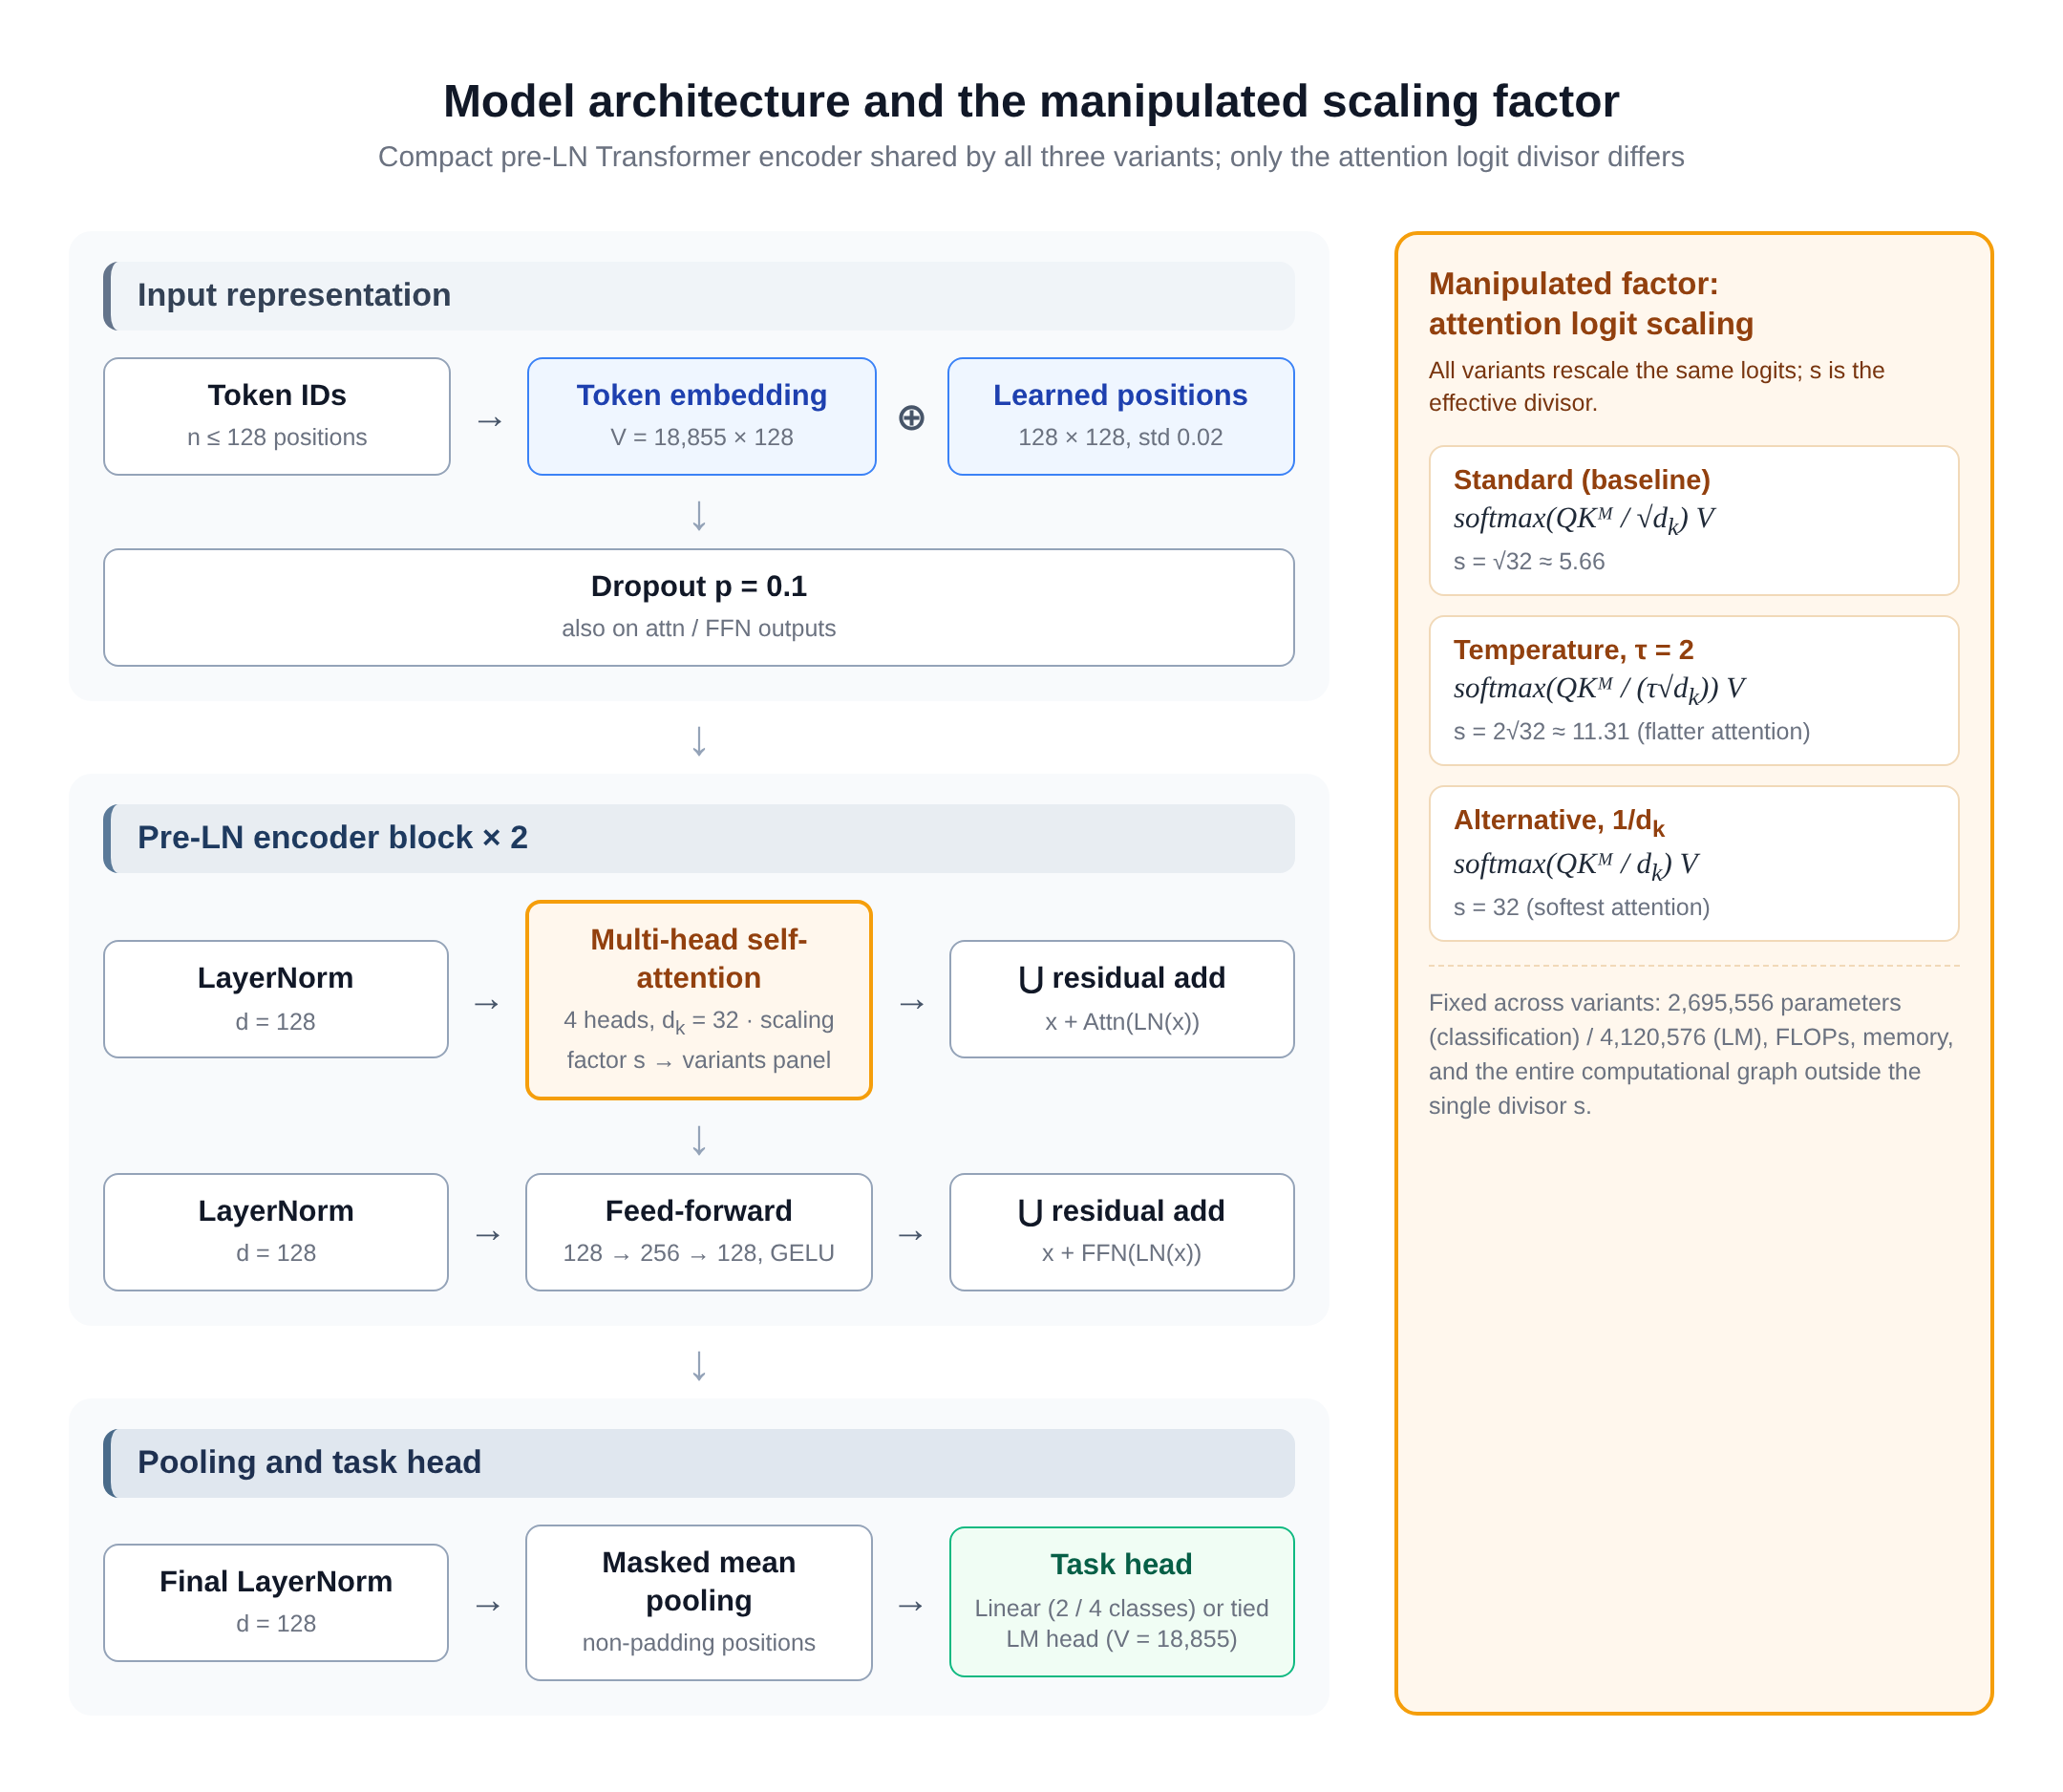
\includegraphics[width=0.94\textwidth]{figures/fig_architecture.png}
  \caption{Model architecture and the manipulated factor. \textbf{Left:} the
  compact pre-LN encoder shared by all variants (2 blocks, 4 heads,
  $\dk = 32$). \textbf{Right:} the three scaling variants, which differ only in
  the effective divisor $s$ of the attention logits. Parameter counts, FLOPs,
  and memory are identical across variants.}
  \label{fig:arch}
\end{figure}

\begin{table}[t]
  \centering
  \caption{Model and optimisation specification (identical for all variants).}
  \label{tab:model}
  \small
  \begin{tabular*}{\textwidth}{@{\extracolsep{\fill}} l l l}
    \toprule
    \textbf{Component} & \textbf{Value} & \textbf{Notes} \\
    \midrule
    Vocabulary / max.\ sequence length & 18{,}855 / 128 & built from training data only \\
    $d_{\text{model}}$ / heads / $\dk$ & 128 / 4 / 32 & per-head dimension \\
    Encoder layers / FFN width & 2 / 256 & pre-LN residual ordering \\
    Projections $W_q, W_k, W_v, W_o$ & $128 \times 128$, bias-free & per block \\
    Activation / dropout & GELU / $p = 0.1$ & \cite{hendrycks2016,srivastava2014} \\
    Pooling & masked mean & non-padding positions \\
    Task head & Linear (2/4 classes) or tied LM head & WikiText-2: weight-tied \\
    Attention logit clamp & $[-50, 50]$ & numerical stability \\
    Parameter count & 2{,}695{,}556 (cls) / 4{,}120{,}576 (LM) & identical across variants \\
    \midrule
    Optimiser & AdamW \cite{loshchilov2019} & $\beta = (0.9, 0.999)$, $\epsilon = 10^{-8}$ \\
    Learning rate / weight decay & $3 \times 10^{-4}$ / 0.01 & \cite{kingma2015} \\
    LR schedule & linear warmup (5\% of steps), cosine decay & \\
    Batch size & 64 (classification) / 16 (LM) & eval.\ 64 / 32 \\
    Gradient clipping & $\max\|g\|_2 = 1.0$ & \\
    Precision & FP32 (mixed precision disabled) & reproducibility \\
    Budgets & 2 epochs (core) / 25 epochs (extended) / 25{,}000 steps (LM) & frozen per grid \\
    \bottomrule
  \end{tabular*}
\end{table}

\subsection{Datasets and preprocessing}\label{sec:datasets}
Four datasets span two task families (Table~\ref{tab:datasets}): topic
classification (AG News, 4 classes \cite{zhang2015}), sentiment classification
(SST-2 \cite{socher2013} and IMDB \cite{maas2011}), and language modelling
(WikiText-2 \cite{merity2017}). All datasets are loaded through the HuggingFace
\texttt{datasets} ecosystem \cite{wolf2020} with fixed splits: classification
training sets are subsampled to 10{,}000 examples with a 20\% held-out
validation split (SST-2 uses the official GLUE validation and test splits), and
WikiText-2 is tokenised into 128-token sequences. Classification text is
tokenised with a lowercased regular-expression pattern (\texttt{[a-z0-9']+});
language modelling uses whitespace tokenisation with an end-of-sequence token.
Vocabularies (top 18{,}855 tokens at minimum frequency 2) are built from
training data only, so no test information leaks into preprocessing. Sequences
are right-padded to length 128 with attention masks that exclude padding
positions.

\begin{table}[t]
  \centering
  \caption{Datasets and splits. Classification training sets are subsampled to
  10{,}000 examples; validation splits follow the repository configuration.}
  \label{tab:datasets}
  \small
  \begin{tabular*}{\textwidth}{@{\extracolsep{\fill}} l l l r r r l}
    \toprule
    \textbf{Dataset} & \textbf{Task} & \textbf{Classes} & \textbf{Train} &
    \textbf{Val} & \textbf{Test} & \textbf{Source} \\
    \midrule
    AG News    & topic classification & 4 & 10{,}000 & 2{,}000 & 7{,}600  & \cite{zhang2015} \\
    SST-2      & sentiment classification & 2 & 10{,}000 & 1{,}115 & 1{,}821 & \cite{socher2013} \\
    IMDB       & sentiment classification & 2 & 10{,}000 & 2{,}000 & 25{,}000 & \cite{maas2011} \\
    WikiText-2 & language modelling &~--- & 36{,}718 seq & 3{,}760 seq & 4{,}358 seq & \cite{merity2017} \\
    \bottomrule
  \end{tabular*}
\end{table}

\subsection{Matched-seed paired design}\label{sec:design}
The core classification grid is 3 variants $\times$ 25 seeds $\times$ 3 datasets
$= 225$ runs at GPU scale; the language-modelling grid (3 variants $\times$
25 seeds) is completed in Stage 2 at replica scale with the corrected causal
mask (Section~\ref{sec:replica-protocol}). Within a seed $s \in \{1001, \dots,
1025\}$, the three variants share (i) a bit-identical parameter initialization
$\theta_0(s)$~--- verified by unit tests that compare initial-state hashes
across variants, (ii) the same training-example order driven by a seeded
permutation generator, (iii) the same optimizer state trajectory shape, and
(iv) the same frozen budget (Figure~\ref{fig:design}). The unit of statistical
analysis is therefore the within-seed difference $d(s) = a_{\text{std}}(s) -
a_v(s)$, giving $n = 25$ paired observations per comparison. This design removes
initialization and data-order variance~--- typically the dominant variance
components in small-model training \cite{bouthillier2021}~--- from the
comparison, and it is exactly the matched-pair structure recommended for NLP
evaluation \cite{dror2018}.

\begin{figure}[t]
  \centering
  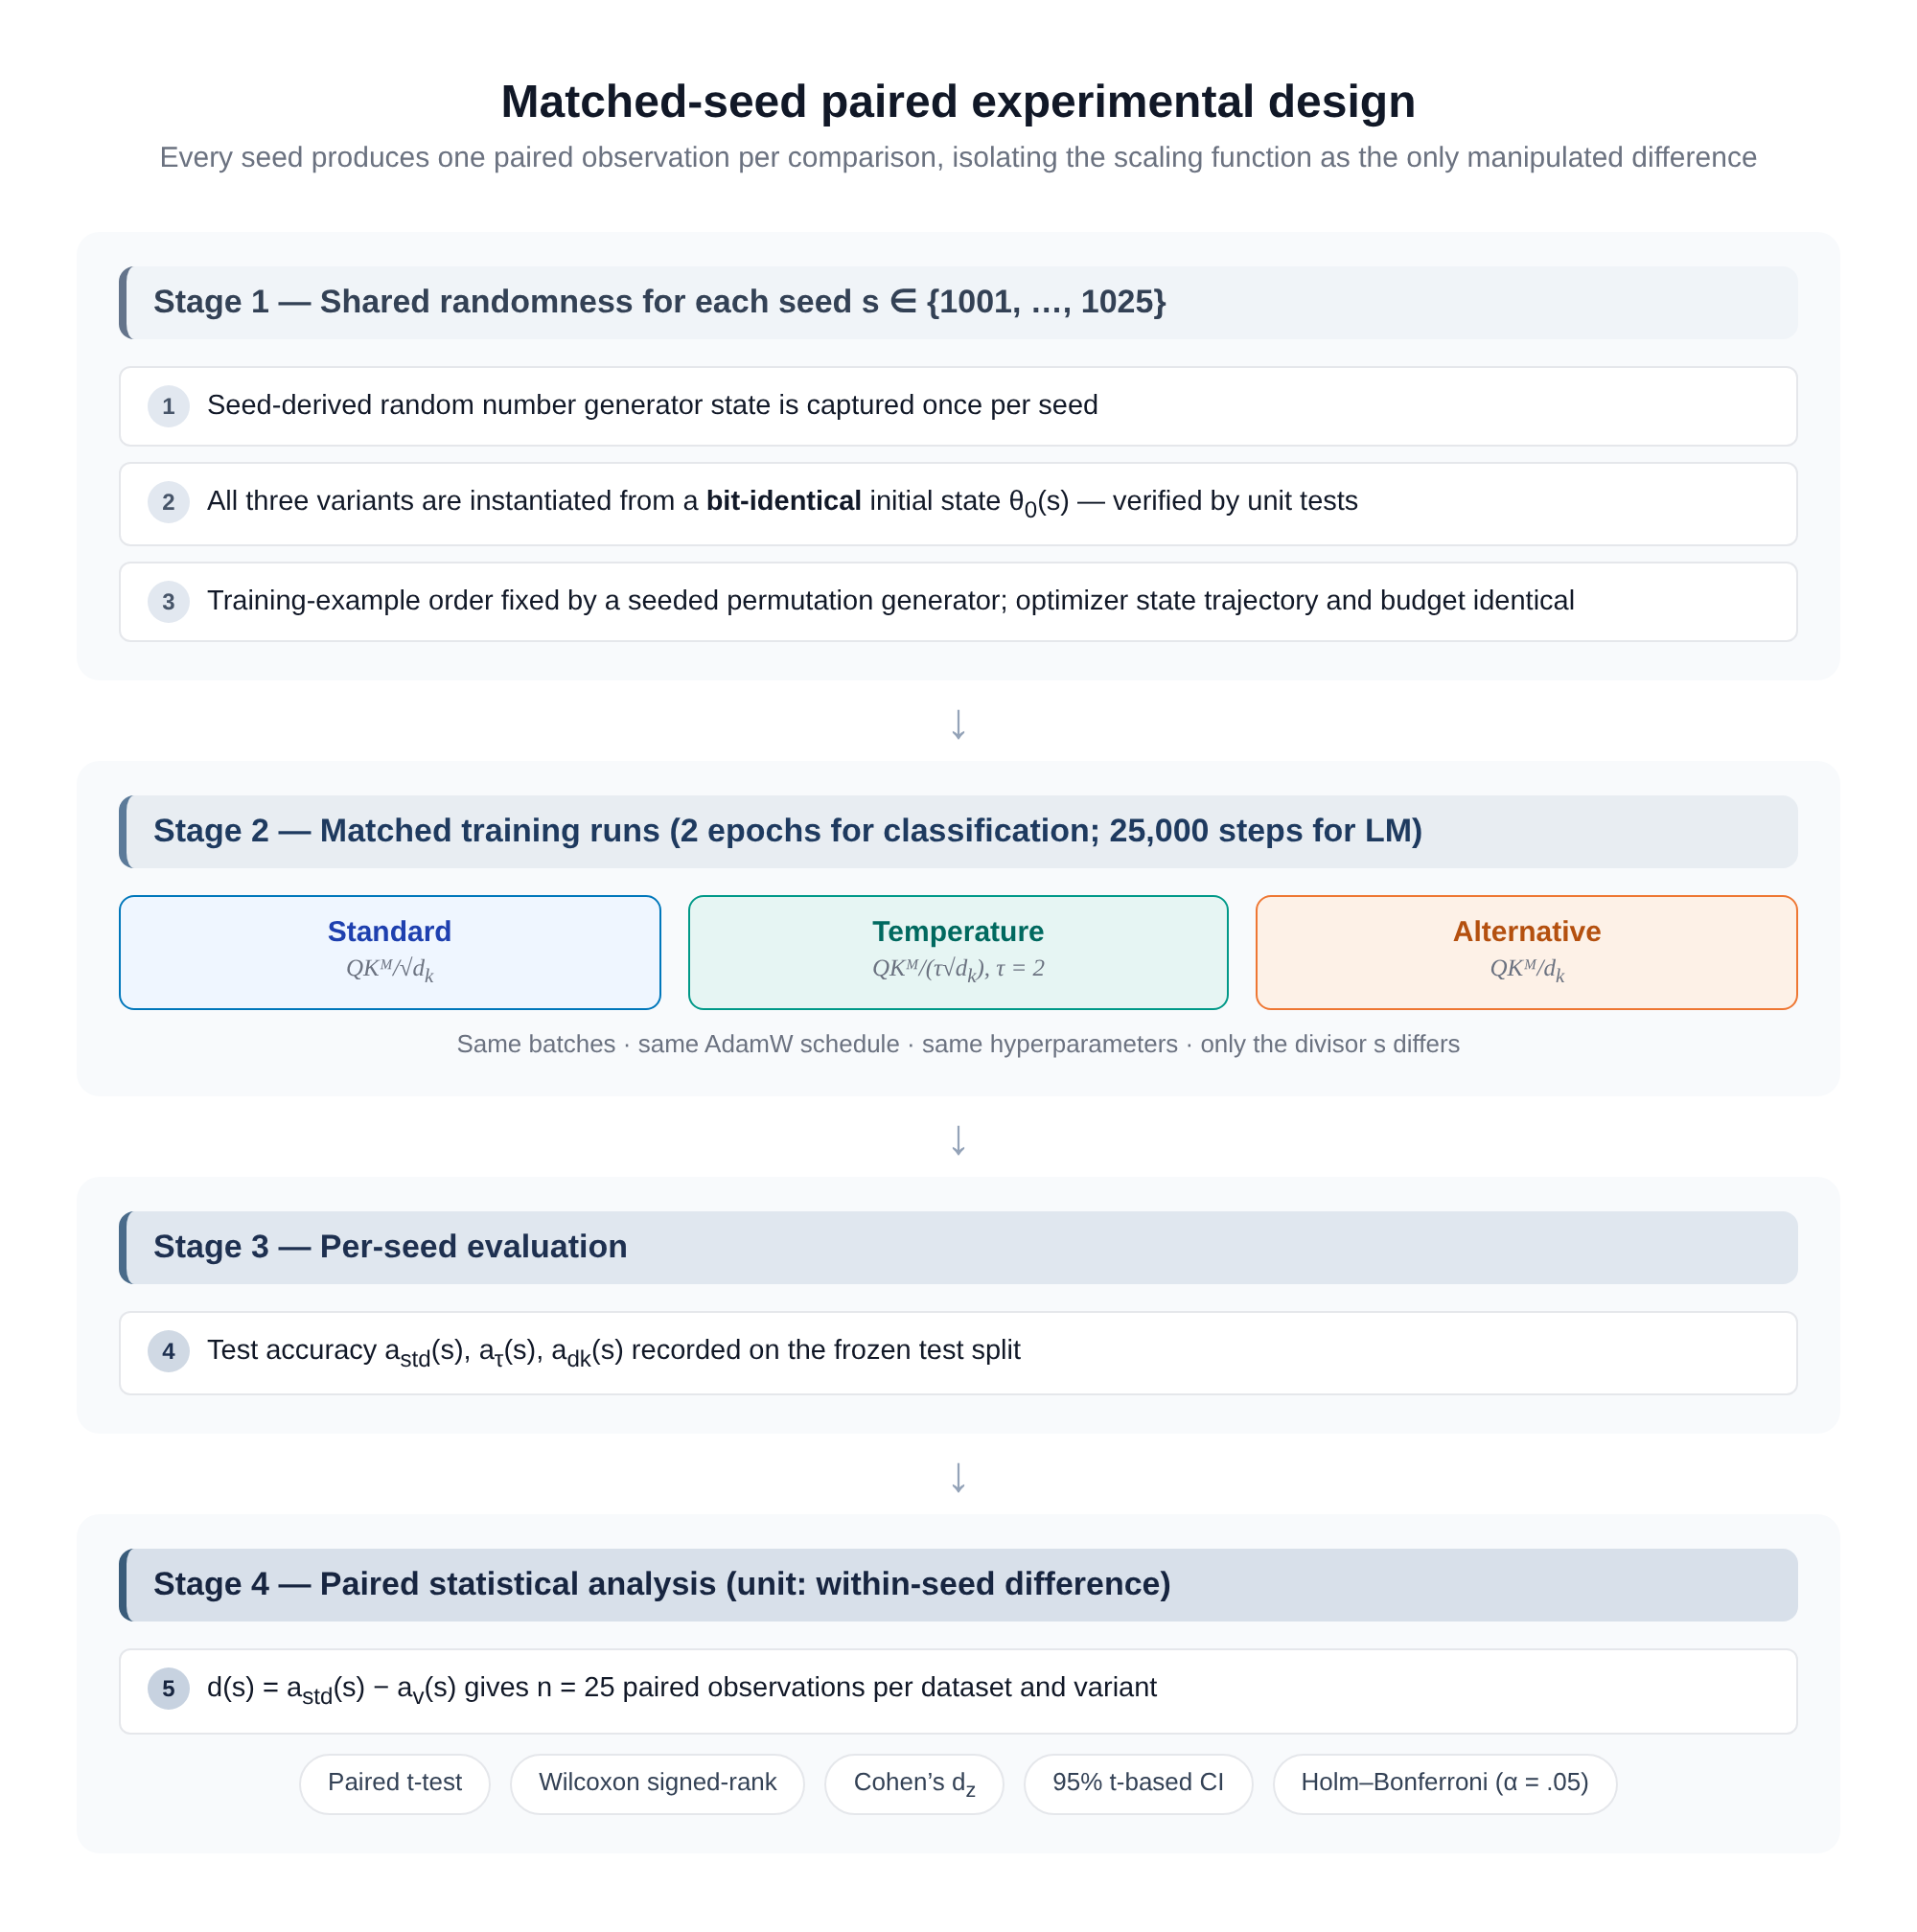
\includegraphics[width=0.9\textwidth]{figures/fig_design.png}
  \caption{Matched-seed paired experimental design. Each seed contributes one
  paired observation per comparison, so the scaling function is the only
  manipulated difference between arms.}
  \label{fig:design}
\end{figure}

\subsection{Stage-2 replica protocol and artifact probes}\label{sec:replica-protocol}
Stage 2 completes the grids that Stage 1 left open on a documented replica
protocol, chosen to fit a 2-core CPU sandbox (3\,GB RAM, PyTorch 2.15 CPU
build) while preserving every structural property of the design: the same
pre-LN architecture, the same three scaling variants with the same effective
divisors, the same matched-seed construction (bit-identical initial state,
shared data order), the same optimizer (AdamW, $\mathrm{lr}=3\times10^{-4}$,
weight decay 0.01, 5\% linear warmup then cosine decay, gradient clip 1.0),
and the same analysis pipeline. The reductions are: 2{,}000-example training
subsets (val 500; test sets 4{,}000/872/2{,}500 for AG News/SST-2/IMDB),
64-token sequences, batch 32, and per-dataset word-level vocabularies built on
the training subset (AG News 7{,}234; SST-2 2{,}249; IMDB 12{,}000; WikiText-2
5{,}655 with 96{,}000 training tokens and 40{,}000 validation tokens). The
replica LM uses $d_{\text{model}}{=}96$, 3 heads ($d_k{=}32$), 2 layers,
$d_{\text{ff}}{=}192$, batch 32, 3 epochs; the classification replica keeps the
original $d_{\text{model}}{=}128$, 4 heads. Seed allocation is 1001--1025 for
the replica core and LM, 1001--1012 for the $\dk$ grid, 1001--1005 for
train-to-convergence, and 1001--1003 for the ablations. Every run is recorded
as an append-only JSONL record keyed by (phase, dataset, variant, $\dk$, seed),
making the grid resume-safe and auditable; 312 pre-registered runs completed
without gaps, plus 27 mask-artifact probes (Section~\ref{sec:lm}).

\subsection{Stage-3 operating-point protocol}\label{sec:stage3-protocol}
Stage 3 manipulates the softmax operating point directly. All arms reuse the
replica architecture, matched-seed construction, and JSONL record protocol of
Section~\ref{sec:replica-protocol}; the new mechanisms are four.
\emph{(i) Divisor power law.} For i.i.d.\ $N(0, \sigma^2)$ logits over $n$
attended positions, the KL divergence between the attention distributions
induced by two divisors is derived to second order in $(b\,\sigma)$
($b = 1/c$; Appendix S17 of the supplementary material) and validated by Monte Carlo
(200{,}000 replicates per grid point; $\dk \in \{32, 128\}$,
$n \in \{64, 128\}$, $\sigma \in [0.5, 16]$).
\emph{(ii) Logit gain.} A scalar $g$ multiplies $q$ and $k$ each by
$\sqrt{g}$ after the output projections and before QK-Norm, so the raw logit
variance scales by $g$ while everything else (initialization, data order,
optimizer trajectory shape) is held fixed; the gain sweep uses
$g \in \{1, 2, 4, 8, 16, 32\}$, 4 seeds, 3 variants (72 runs). The
regime-restored arms train 6{,}000-example AG News for 8 epochs with per-epoch
operating-point probes at $\dk \in \{32, 128\}$ (18 runs), and the LM gain arm
trains the replica LM at sequence length 128 with $g \in \{1, 4\}$
(18 runs).
\emph{(iii) Operating-point probe.} Every Stage-3 run records, per layer, the
raw pre-division logit SD $\sigma_{\text{raw}}$, the realised attention
entropy and maximum weight under the model's own divisor, and the KL
divergence between the attention maps the \emph{same} logits would induce
under each of the three divisors~--- the exact quantity
Eq.~\eqref{eq:law} predicts.
\emph{(iv) Frontier stabilisers and pretrained decoders.} The bridge arms add
per-head QK-normalisation (LayerNorm on $q, k$; affine defaults preserve
bit-identical matched initialization) and Gemma-2-style attention logit
soft-capping ($z \mapsto c \tanh(z/c)$, $c = 3.0$) at gain 32 (20 runs). The
frontier probe loads pretrained GPT-2 checkpoints (124M, 355M) with eager
attention, replaces only the attention scaling factor
($1/\sqrt{d_k} \to 1/d_k$ or $1/(2\sqrt{d_k})$; $d_k = 64$), and evaluates
WikiText-2 validation perplexity over 160 non-overlapping 128-token windows
with per-layer $\sigma_{\text{raw}}$, entropy, and KL diagnostics (6
evaluations). A companion GPU script extends the identical intervention and
diagnostics to 1B--7B HuggingFace decoders (GPT-2-XL, Pythia, Llama-3.2,
Qwen2.5) and is shipped with the repository
(\texttt{scripts/frontier/frontier\_gpu\_1b7b.py}).

\subsection{Statistical analysis}\label{sec:stats}
For each dataset and variant $v$ we compute the paired differences
$d_i = a_{\text{std}}(s_i) - a_{v}(s_i)$, $i = 1, \dots, n$, and report the mean
difference, the 95\% $t$-based confidence interval
\begin{equation}\label{eq:ci}
  \bar d \;\pm\; t_{0.975,\,n-1} \cdot \frac{\operatorname{SD}(d)}{\sqrt{n}},
\end{equation}
Cohen's $d_z$ for paired designs,
\begin{equation}\label{eq:dz}
  d_z \;=\; \frac{\bar d}{\operatorname{SD}(d)},
\end{equation}
with conventional magnitude labels (negligible $|d_z| < 0.2$, small, medium,
large) \cite{cohen1988}, the two-sided paired $t$-test, and the Wilcoxon
signed-rank test as a non-parametric confirmation \cite{wilcoxon1945}. Because
each dataset contributes two comparisons against the common baseline, family-wise
error is controlled with the Holm--Bonferroni step-down procedure
\cite{holm1979} within each dataset at $\alpha = 0.05$. Effect sizes and
confidence intervals are interpreted with the usual cautions for small samples.

\subsection{Implementation, validation, and reproducibility}\label{sec:impl}
The study is implemented in PyTorch with configuration-driven experiment scripts
(YAML), a preflight validator that checks the environment and configurations
before launch, and 22 unit tests in 5 suites covering: bit-identical
initialization across variants for a fixed seed, gradient flow through all
variants, output shapes, masked attention correctness, and data-pipeline
determinism. Mixed precision is disabled and logits are clamped to $[-50, 50]$
for numerical stability. Every run writes a per-seed JSON record (configuration
hash, training history, and test metrics) from which the aggregate tables and
figures in this paper are generated by committed analysis scripts. The full
package~--- source, configurations, tests, per-seed records, statistical
analysis outputs, figures, and this manuscript~--- is released under an MIT
licence.\footnote{\url{https://github.com/razahasan2000/Attention-Scaling}}

% ============================================================================
% 4. Results
% ============================================================================
\section{Results}\label{sec:results}

\subsection{The completed three-stage programme}\label{sec:manifest}
The experimental programme is now complete and proceeds in three stages.
\emph{Stage 1} is the original GPU-scale study: a compact pre-LN encoder
($d_{\text{model}}=128$, 4 heads, $d_k=32$) trained on the full training
subsets (10{,}000 examples, 128-token sequences, batch 64) for 2 epochs, plus
the temperature ablation, an extended 25-epoch budget, and the original
language-modelling runs. \emph{Stage 2}, reported in this revision, completes
every grid that Stage 1 left open, on a documented replica protocol (2-core CPU
sandbox; 2{,}000-example training subsets, 64-token sequences, batch 32; full
specification in Sections~\ref{sec:replica-protocol}
and~S13 of the supplementary material): the 25-seed replica core, the corrected causal-mask
language-modelling grid (25 seeds $\times$ 3 variants), the head-dimension grid
$\dk \in \{32, 64, 128\}$, train-to-convergence with early stopping, and
multi-seed E1--E4 ablations. \emph{Stage 3}, also reported in this revision,
responds to the operating-point diagnosis of Section~\ref{sec:scale}: it
quantifies the regime in which the divisor can act at all (a power law,
validated by Monte Carlo), then deliberately moves the operating point into
that regime three ways~--- an injected logit gain, longer training at two head
dimensions, and inference-time divisor swaps in a pretrained decoder~--- and
adds the frontier stabilisers (QK-Norm, soft-capping) under which large logits
are tolerated in practice. All stages share the same matched-seed paired
design, statistical machinery, and analysis scripts.
In total the programme comprises 787 runs: 314 at GPU scale, 339 at replica
scale (312 pre-registered completions plus 27 mask-artifact probes), and 134
in the Stage-3 operating-point programme (128 matched-seed training runs plus
6 pretrained-model evaluations).

\begin{table}[t]
  \centering
  \caption{Completed experiment manifest. Stage 1 = GPU-scale protocol;
  Stage 2 = replica-scale completion; Stage 3 = operating-point programme
  (this revision). Every preregistered grid is complete in at least one
  stage.}
  \label{tab:manifest}
  \small
  \begin{tabular*}{\textwidth}{@{\extracolsep{\fill}} l l l r}
    \toprule
    \textbf{Grid} & \textbf{Design} & \textbf{Stage} & \textbf{Runs} \\
    \midrule
    Core classification & 3 variants $\times$ 25 seeds $\times$ 3 datasets & 1 & 225 \\
    Temperature ablation & 4 temperatures $\times$ 3 seeds $\times$ 2 datasets & 1 & 24 \\
    Extended budget & 3 variants $\times$ 5 seeds $\times$ 2 datasets, 25 epochs & 1 & 30 \\
    Core language modelling & 3 variants $\times$ 25 seeds (v1 protocol) & 1 & 25 \\
    Focused ablations E1--E4 & single-seed arms, 5 epochs & 1 & 10 \\
    \midrule
    Replica core classification & 3 variants $\times$ 25 seeds, AG News & 2 & 75 \\
    Replica language modelling & 3 variants $\times$ 25 seeds, corrected causal mask & 2 & 75 \\
    Head-dimension grid & $\dk \in \{32,64,128\}$ $\times$ 3 variants $\times$ 12 seeds & 2 & 108 \\
    Train-to-convergence & 3 variants $\times$ 5 seeds $\times$ 2 datasets, early stopping & 2 & 30 \\
    Replica ablations E1--E4 & 4 arms $\times$ 3 seeds $\times$ 2 datasets, 5 epochs & 2 & 24 \\
    Mask-artifact probes & leaky vs.\ causal, 3 and 10 epochs & 2 & 27 \\
    \midrule
    Logit-gain sweep & $g \in \{1,2,4,8,16,32\}$ $\times$ 3 variants $\times$ 4 seeds & 3 & 72 \\
    Regime-restored AG News & 6{,}000 train, 8 epochs, per-epoch probes, $\dk \in \{32,128\}$ & 3 & 18 \\
    Frontier-stabiliser bridge & QK-Norm / soft-cap arms $\times$ 4 seeds & 3 & 20 \\
    LM logit gain & $g \in \{1,4\}$ $\times$ 3 variants $\times$ 3 seeds, seq 128 & 3 & 18 \\
    Frontier divisor swap & GPT-2 + GPT-2-medium, inference-time, 3 divisors & 3 & 6 \\
    \midrule
    \textbf{Total} & & & \textbf{787} \\
    \bottomrule
  \end{tabular*}
\end{table}

\subsection{Stage 1: GPU-scale core comparison}\label{sec:main-results}
Figure~\ref{fig:main} and Table~\ref{tab:core} present test accuracy across the
25-seed core grid. On AG News, standard scaling reached 91.23\% ($\pm 0.25$),
versus 91.13\% ($\pm 0.26$) for the temperature variant $\tau = 2$ and 90.92\%
($\pm 0.32$) for $1/\dk$~--- a strictly ordered pattern in which softening the
attention distribution monotonically hurt. On the binary sentiment tasks the
ordering vanished: SST-2 accuracies fell within 0.08\,\pp{} of one another and
IMDB accuracies within 0.04\,\pp, with overlapping seed distributions
(Figure~\ref{fig:main}, middle and right).

\begin{figure}[t]
  \centering
  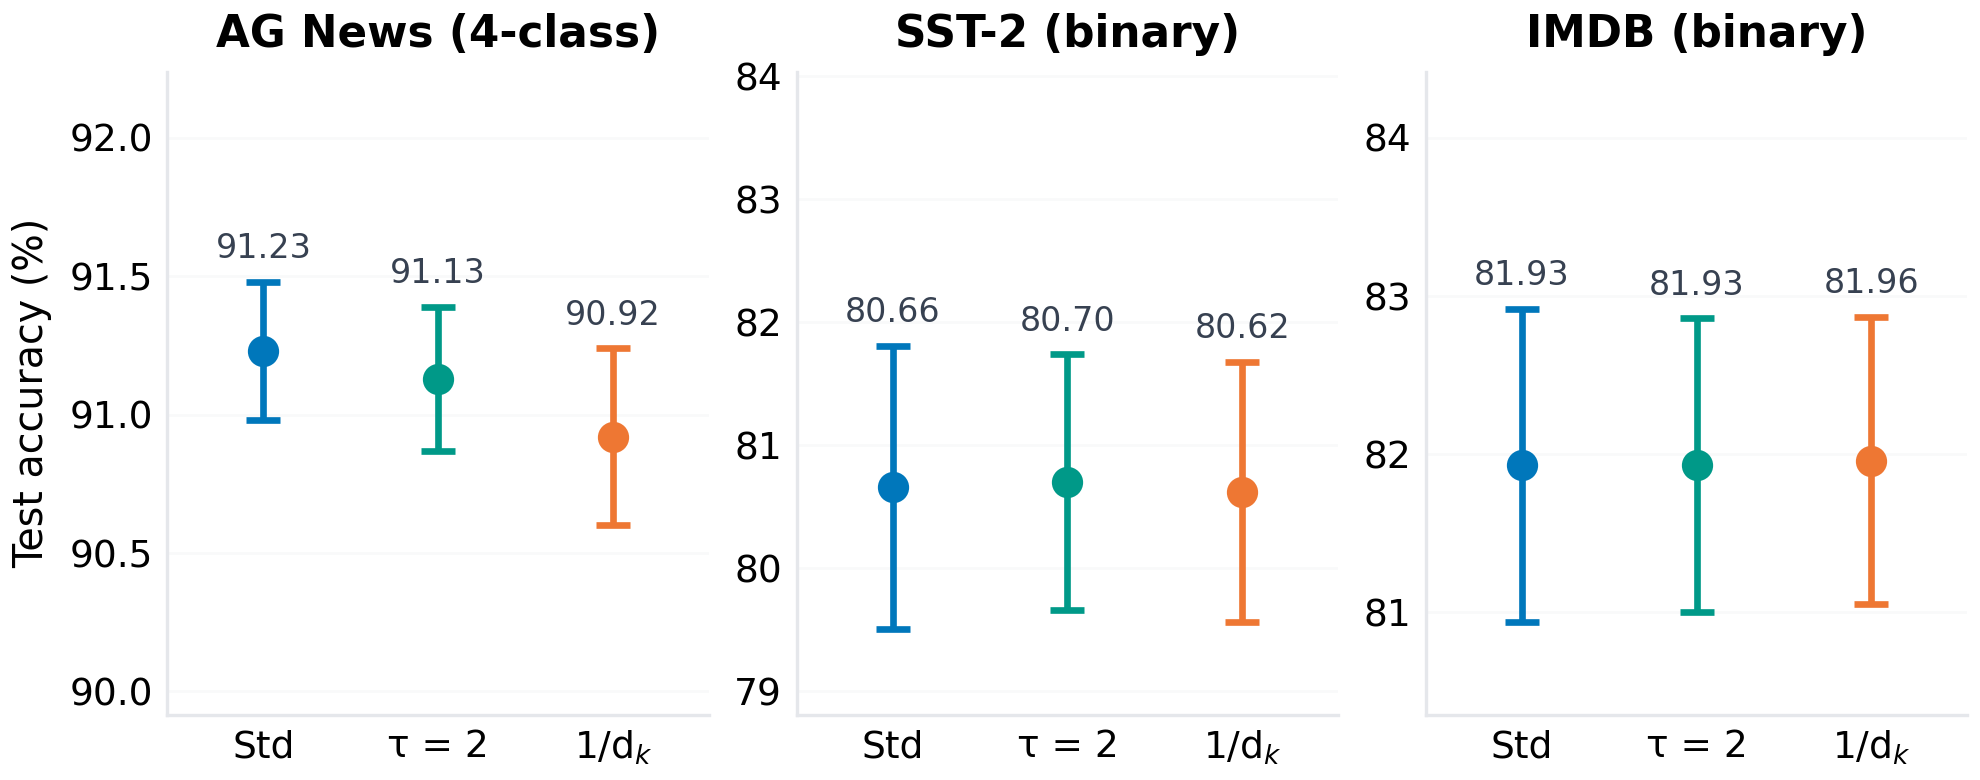
\includegraphics[width=\textwidth]{figures/fig_main_performance.png}
  \caption{Core-grid test accuracy (mean $\pm$ one standard deviation across 25
  matched seeds, 2-epoch budget). Only AG News shows a strictly ordered, visibly
  separated pattern; on SST-2 and IMDB the seed distributions overlap almost
  completely.}
  \label{fig:main}
\end{figure}

\begin{table}[t]
  \centering
  \caption{Core-grid results, Stage 1 (25 matched seeds, 2-epoch GPU budget;
  language-modelling rows are the superseded v1 leaky-mask values, see
  Section~\ref{sec:lm}). $\pm$ denotes one standard deviation across seeds;
  CI is the 95\% confidence interval of the mean.}
  \label{tab:core}
  \small
  \begin{tabular*}{\textwidth}{@{\extracolsep{\fill}} l l r r c r}
    \toprule
    \textbf{Dataset} & \textbf{Variant} & \textbf{Mean} & \textbf{$\pm$ SD} &
    \textbf{95\% CI} & \textbf{$n$} \\
    \midrule
    \multirow{3}{*}{AG News (\%)} & Standard & 91.23 & 0.25 & $[91.13, 91.33]$ & 25 \\
      & Temp ($\tau=2$) & 91.13 & 0.26 & $[91.03, 91.24]$ & 25 \\
      & $1/\dk$ & 90.92 & 0.32 & $[90.80, 91.04]$ & 25 \\
    \midrule
    \multirow{3}{*}{SST-2 (\%)} & Standard & 80.66 & 1.15 & $[80.19, 81.13]$ & 25 \\
      & Temp ($\tau=2$) & 80.70 & 1.04 & $[80.27, 81.13]$ & 25 \\
      & $1/\dk$ & 80.62 & 1.06 & $[80.18, 81.06]$ & 25 \\
    \midrule
    \multirow{3}{*}{IMDB (\%)} & Standard & 81.93 & 0.99 & $[81.52, 82.34]$ & 25 \\
      & Temp ($\tau=2$) & 81.93 & 0.93 & $[81.55, 82.31]$ & 25 \\
      & $1/\dk$ & 81.96 & 0.91 & $[81.58, 82.34]$ & 25 \\
    \midrule
    \multirow{3}{*}{WikiText-2 (ppl $\downarrow$, v1 artefact$^\dagger$)} & Standard & 1.0917 & 0.0061 & $[1.089, 1.095]$ & 15 \\
      & Temp ($\tau=2$) & 1.0882 & 0.0056 & $[1.083, 1.093]$ & 7 \\
      & $1/\dk$ & 1.0809 & 0.0021 & $[1.077, 1.085]$ & 3 \\
    \bottomrule
    \multicolumn{6}{l}{\footnotesize $^\dagger$Historical v1 values under the leaky (non-causal) mask; superseded by the corrected
    protocol in Table~\ref{tab:lm}.}
  \end{tabular*}
\end{table}

\subsection{Paired differences and effect sizes (Stage 1)}\label{sec:paired}
Because the design is seed-matched, the informative statistics are the paired
differences of Table~\ref{tab:paired} and Figure~\ref{fig:paired}. On AG News,
standard scaling beat $1/\dk$ by $+0.31$\,\pp{} (95\% CI $[0.22, 0.39]$, $d_z =
1.52$, $t(24) = 7.60$, $p_{\text{Holm}} < 0.001$) and beat $\tau = 2$ by
$+0.10$\,\pp{} (95\% CI $[0.02, 0.17]$, $d_z = 0.53$, $t(24) = 2.65$,
$p_{\text{Holm}} = 0.013$)~--- large and medium paired effect sizes
respectively \cite{cohen1988}. Wilcoxon signed-rank tests confirmed both
directions. On SST-2 and IMDB all four comparisons had confidence intervals
straddling zero and negligible effect sizes ($|d_z| \le 0.19$,
$p_{\text{Holm}} \ge 0.70$). In other words, the AG News effect is not an
artefact of seed luck: it appears in the matched within-seed contrasts, where
initialization and data order are held constant.

\begin{table}[t]
  \centering
  \caption{Paired statistics versus the standard baseline (unit: within-seed
  difference, $n = 25$). Positive differences favour standard scaling.
  $p_{\text{Holm}}$ is Holm--Bonferroni corrected across the two comparisons
  within each dataset. Significance codes: $^{***}\,p < 0.001$,
  $^{*}\,p < 0.05$ after correction.}
  \label{tab:paired}
  \small
  \begin{tabular*}{\textwidth}{@{\extracolsep{\fill}} l l c c c c c c}
    \toprule
    \textbf{Dataset} & \textbf{Comparison} & \textbf{$\Delta$ (pp)} &
    \textbf{95\% CI (pp)} & \textbf{$d_z$} & \textbf{$t(24)$} &
    \textbf{$p_{\text{Holm}}$} & \textbf{Sig.} \\
    \midrule
    AG News & $1/\dk$ vs.\ std & $+0.31$ & $[+0.22, +0.39]$ & $1.52$ & $7.60$ & $<0.001$ & $^{***}$ \\
            & $\tau=2$ vs.\ std & $+0.10$ & $[+0.02, +0.17]$ & $0.53$ & $2.65$ & $0.013$ & $^{*}$ \\
    \midrule
    SST-2   & $1/\dk$ vs.\ std & $+0.04$ & $[-0.23, +0.31]$ & $0.06$ & $0.30$ & $0.781$ & \\
            & $\tau=2$ vs.\ std & $-0.05$ & $[-0.31, +0.21]$ & $-0.07$ & $-0.35$ & $0.718$ & \\
    \midrule
    IMDB    & $1/\dk$ vs.\ std & $-0.04$ & $[-0.11, +0.04]$ & $-0.19$ & $-0.95$ & $0.703$ & \\
            & $\tau=2$ vs.\ std & $-0.01$ & $[-0.06, +0.05]$ & $-0.04$ & $-0.20$ & $0.831$ & \\
    \bottomrule
  \end{tabular*}
\end{table}

\begin{figure}[t]
  \centering
  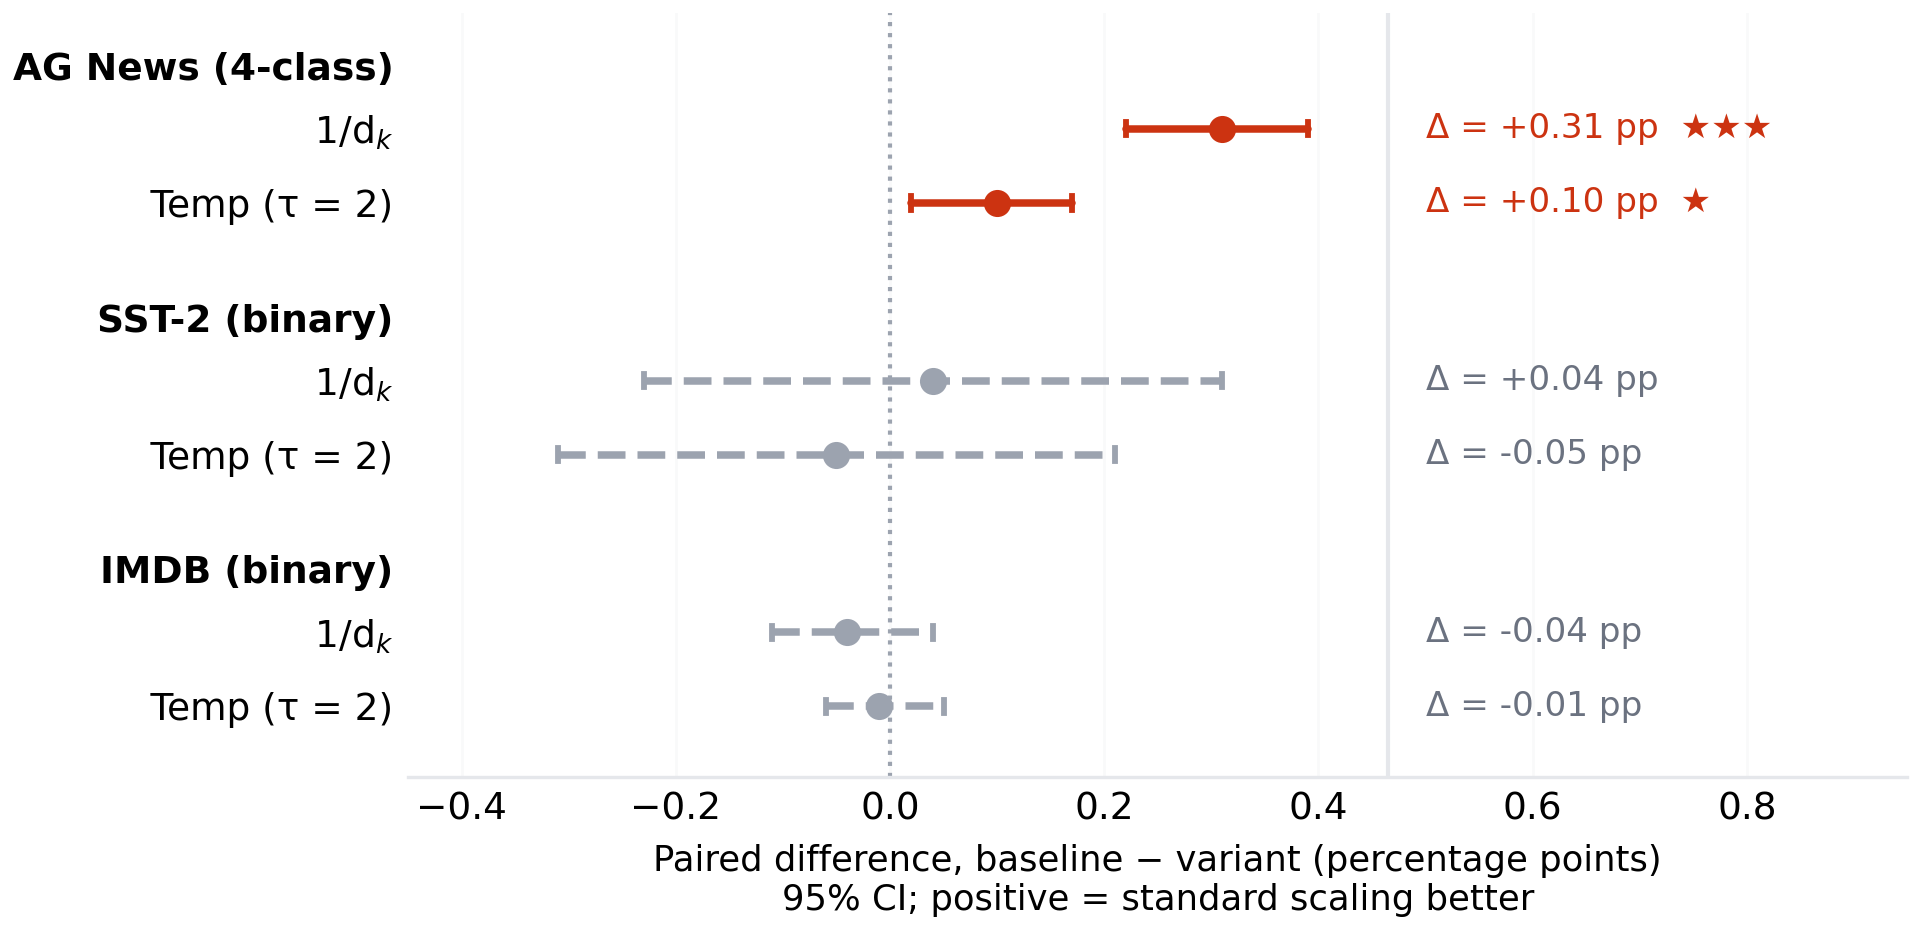
\includegraphics[width=0.96\textwidth]{figures/fig_paired_differences.png}
  \caption{Seed-matched paired differences with 95\% confidence intervals.
  Only the two AG News comparisons (red) exclude zero after Holm--Bonferroni
  correction; all SST-2 and IMDB intervals (grey) straddle zero.}
  \label{fig:paired}
\end{figure}

\subsection{Stage 2: replica completion of the core grid}\label{sec:replica}
The first Stage-2 question is whether the AG News effect of Section~\ref{sec:paired}
survives a fivefold reduction in training data and sequence length. Under the
replica protocol (2{,}000 training examples, 64-token sequences, otherwise
identical architecture and matched-seed design), all three variants land within
0.01\,\pp{} of one another: 78.51\% ($\pm 1.26$) for standard scaling, 78.51\%
($\pm 1.25$) for $\tau = 2$, and 78.50\% ($\pm 1.24$) for $1/\dk$
(Figure~\ref{fig:replica}a, Table~\ref{tab:replica}). The paired differences
are $-0.01$\,\pp{} (95\% CI $[-0.04, +0.02]$, $d_z = -0.13$) for $1/\dk$ versus
standard and $+0.00$\,\pp{} ($d_z = 0.04$) for $\tau=2$ versus standard; both
$p_{\text{Holm}} = 1.00$ (Figure~\ref{fig:replica}b). The Stage-1 AG News
effect of $+0.31$\,\pp{} therefore does \emph{not} replicate at this operating
point: the replica confidence interval excludes any advantage larger than
0.02\,\pp. We return to the interpretation of this scale dependence in
Section~\ref{sec:scale}.

\begin{figure}[t]
  \centering
  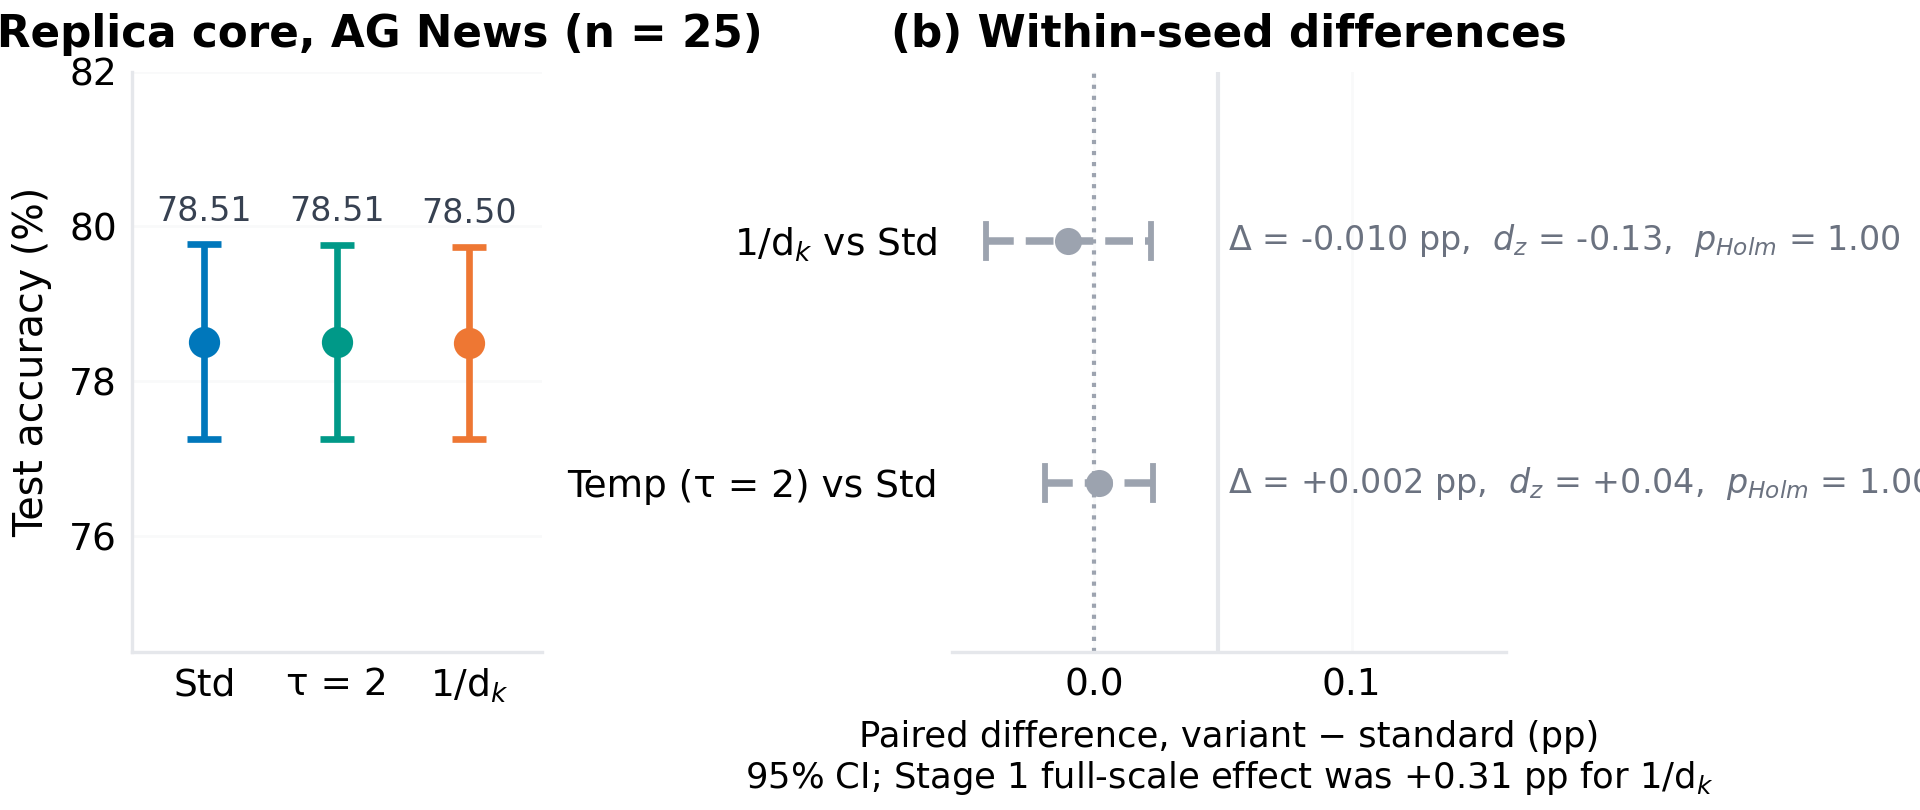
\includegraphics[width=\textwidth]{figures/fig_stage2_core.png}
  \caption{Stage-2 replica core on AG News (25 matched seeds, 2 epochs).
  (a) Test accuracy by variant. (b) Within-seed paired differences with 95\%
  CIs; both intervals straddle zero, and the replica CI excludes the Stage-1
  full-scale effect of $+0.31$\,\pp{} for $1/\dk$.}
  \label{fig:replica}
\end{figure}

\begin{table}[t]
  \centering
  \caption{Stage-2 replica results. Left: AG News core (25 seeds, 2 epochs).
  Right: within-seed paired statistics versus standard ($n=25$);
  $p_{\text{Holm}}$ across the two comparisons.}
  \label{tab:replica}
  \small
  \begin{tabular*}{\textwidth}{@{\extracolsep{\fill}} l r r r l}
    \toprule
    \textbf{Variant} & \textbf{Mean (\%)} & \textbf{$\pm$ SD} & \textbf{$n$} &
    \textbf{Paired vs.\ standard} \\
    \midrule
    Standard & 78.51 & 1.26 & 25 & --- \\
    Temp ($\tau=2$) & 78.51 & 1.25 & 25 & $\Delta = +0.00$ pp, $d_z = 0.04$, $p_{\text{Holm}} = 1.00$ \\
    $1/\dk$ & 78.50 & 1.24 & 25 & $\Delta = -0.01$ pp, $d_z = -0.13$, $p_{\text{Holm}} = 1.00$ \\
    \bottomrule
  \end{tabular*}
\end{table}

\subsection{Stage 2: head-dimension grid ($\dk \in \{32, 64, 128\}$)}\label{sec:grid}
The variance argument behind $\sqrt{\dk}$ \cite{vaswani2017} predicts that the
logit standard deviation grows as $\sqrt{\dk}$ when the divisor is held at its
standard value but as $\dk$ when the divisor is $1/\dk$; the mismatch between
the two scalings should therefore \emph{amplify} with head dimension, making
larger $\dk$ the regime where the 2017 default is most likely to matter. We
tested this directly on AG News with $d_{\text{model}} = 128$ and
$n_{\text{heads}} \in \{4, 2, 1\}$, giving $\dk \in \{32, 64, 128\}$, 3 variants
$\times$ 12 seeds per point (Table~\ref{tab:grid}, Figure~\ref{fig:grid}).
The prediction is not borne out at this operating point: the $1/\dk$-versus-standard
gap is $+0.010$\,\pp{} ($p = 0.63$) at $\dk=32$, $+0.008$\,\pp{} ($p = 0.75$) at
$\dk=64$, and $+0.017$\,\pp{} ($p = 0.56$) at $\dk=128$, and the paired change in
the gap between $\dk=128$ and $\dk=32$ is $-0.006$\,\pp{} (95\% CI $[-0.077,
+0.064]$, $p = 0.85$). The same holds for $\tau = 2$. The mechanism is
measurable: at this scale the trained models' \emph{raw} logit standard
deviation is of order 1 (1.02--1.19 across variants; Section~\ref{sec:diagnostics}),
so after division by $\sqrt{\dk} \in \{5.7, 8, 11.3\}$ or by $\dk \in \{32, 64,
128\}$ every variant operates in the softmax's near-uniform regime, where
rescaling the logits changes almost nothing downstream. The theoretical
amplification only bites once raw logit variance grows past the divisor, which
the Stage-1 full-data protocol approaches but the replica does not.

\begin{figure}[t]
  \centering
  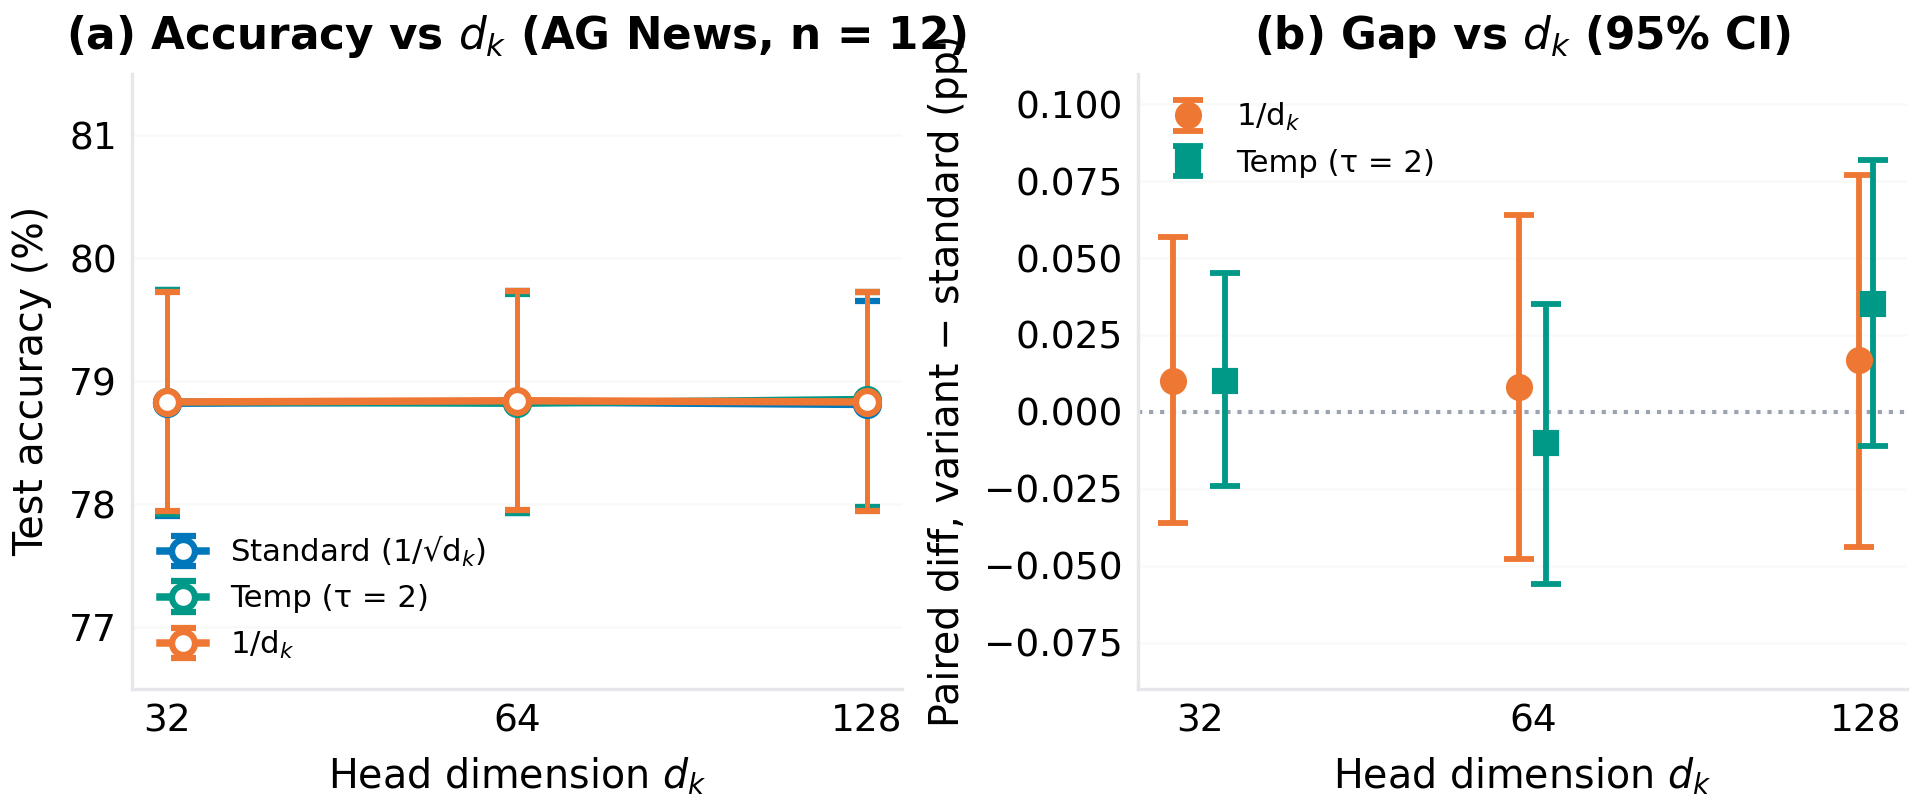
\includegraphics[width=\textwidth]{figures/fig_dk_grid.png}
  \caption{Head-dimension grid on AG News (12 matched seeds per point).
  (a) Test accuracy versus $\dk$ for the three variants. (b) Within-seed gap
  versus standard with 95\% CIs; no trend with $\dk$ (trend $p = 0.85$).}
  \label{fig:grid}
\end{figure}

\begin{table}[t]
  \centering
  \caption{Head-dimension grid, AG News replica (mean $\pm$ SD over 12 seeds;
  within-seed paired differences versus standard).}
  \label{tab:grid}
  \small
  \begin{tabular*}{\textwidth}{@{\extracolsep{\fill}} c c c c c c}
    \toprule
    \textbf{$\dk$} & \textbf{Std (\%)} & \textbf{$\tau{=}2$ (\%)} &
    \textbf{$1/\dk$ (\%)} & \textbf{$\Delta(\tau{=}2)$ (pp)} &
    \textbf{$\Delta(1/\dk)$ (pp)} \\
    \midrule
    32  & 78.82 $\pm$ 0.92 & 78.83 $\pm$ 0.91 & 78.83 $\pm$ 0.89 &
    $+0.01$ ($p{=}0.52$) & $+0.01$ ($p{=}0.63$) \\
    64  & 78.83 $\pm$ 0.90 & 78.82 $\pm$ 0.89 & 78.84 $\pm$ 0.89 &
    $-0.01$ ($p{=}0.63$) & $+0.01$ ($p{=}0.75$) \\
    128 & 78.81 $\pm$ 0.84 & 78.85 $\pm$ 0.87 & 78.83 $\pm$ 0.89 &
    $+0.04$ ($p{=}0.12$) & $+0.02$ ($p{=}0.56$) \\
    \bottomrule
  \end{tabular*}
\end{table}

\subsection{Temperature ablation (Stage 1)}\label{sec:temp-ablation}
The preregistered temperature sweep ($\tau \in \{0.5, 1.0, 1.5, 2.0\}$, 3 seeds
per point, 2 epochs) probes the direction of the effect around the standard
point (Figure~\ref{fig:temp}, Table~\ref{tab:temp}). On SST-2, sharper attention
was monotonically (if noisily) better: $\tau = 0.5$ reached 82.31\% versus
80.77\% for $\tau = 2$~--- a 1.54\,\pp{} spread~--- and on IMDB $\tau = 0.5$
again produced the highest mean (82.29\%), although the $\tau$-response was
flatter. Standard scaling ($\tau = 1$) was intermediate on both datasets. These
3-seed observations are exploratory: confidence intervals are wide (up to
$\pm 1.04$\,\pp{} on SST-2 $\tau = 1.5$), so the sharpest temperature's lead
over the 25-seed core-grid baselines (about $+1.6$\,\pp{} on SST-2) should be
treated as a promising direction rather than an established effect. The
directional pattern is nonetheless consistent with the distillation literature,
where lower temperatures sharpen attention and can help tasks that require
focused token selection \cite{zhang2022temp,hinton2015}.

\begin{figure}[t]
  \centering
  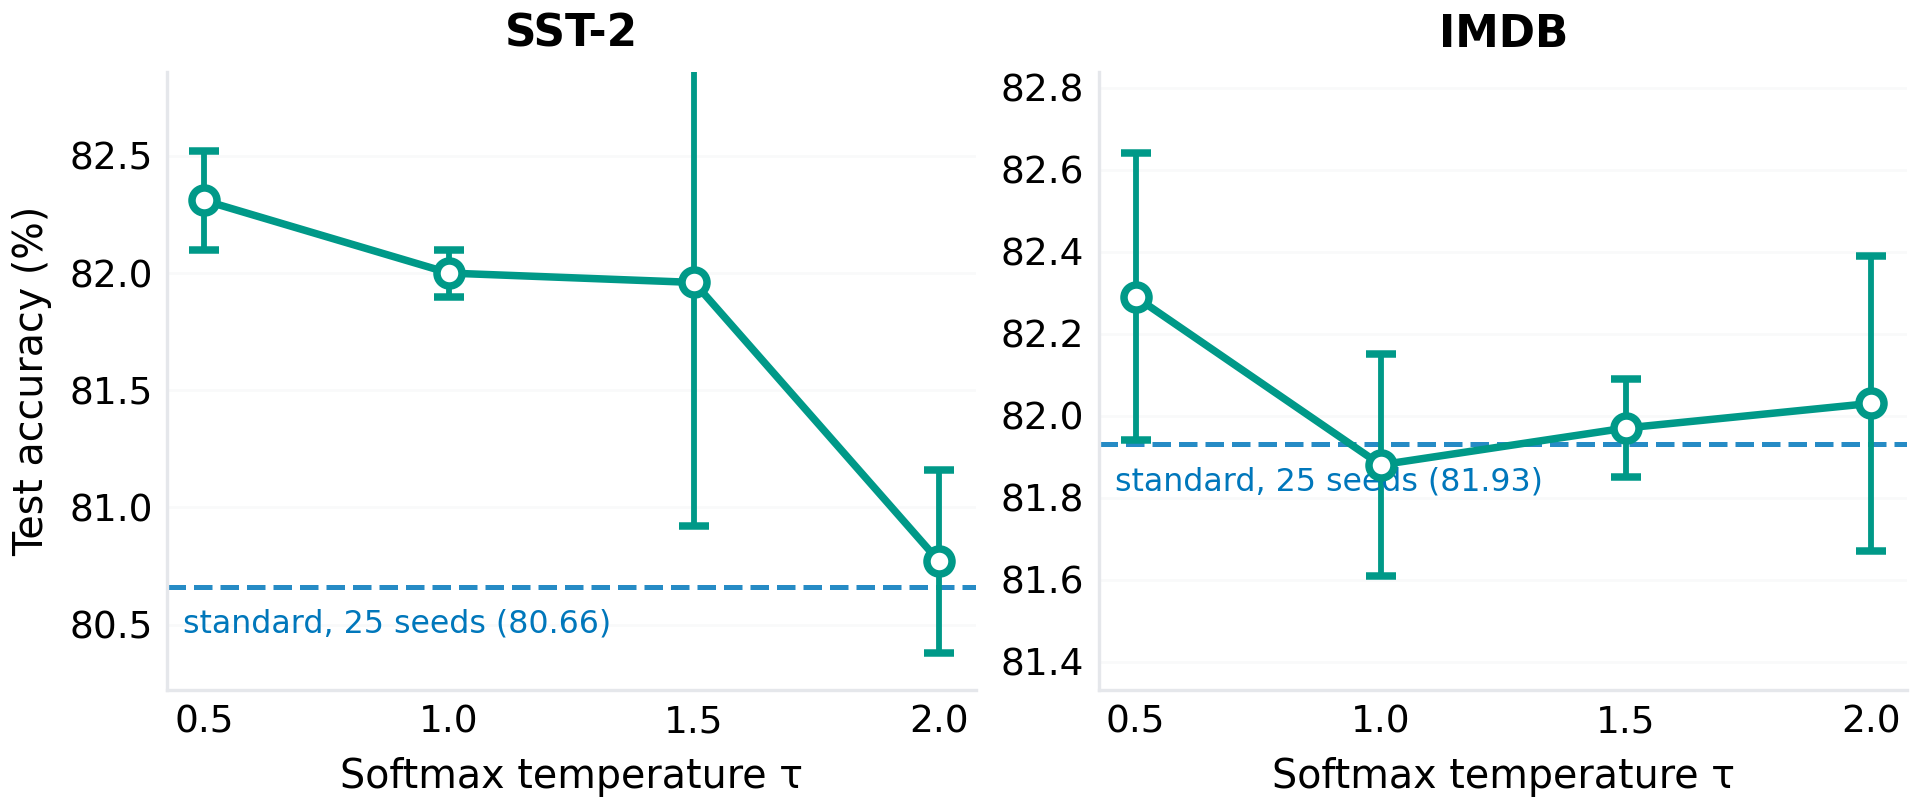
\includegraphics[width=0.9\textwidth]{figures/fig_temperature_ablation.png}
  \caption{Temperature ablation ($n = 3$ seeds per point, 2 epochs; error bars:
  $\pm$ one standard deviation). Dashed reference lines show the 25-seed core
  standard-scaling result at $\tau = 1$.}
  \label{fig:temp}
\end{figure}

\begin{table}[t]
  \centering
  \caption{Temperature ablation results (mean $\pm$ SD across 3 seeds).}
  \label{tab:temp}
  \small
  \begin{tabular*}{0.8\textwidth}{@{\extracolsep{\fill}} l c c c c}
    \toprule
    \textbf{$\tau$} & \textbf{SST-2 (\%)} & \textbf{SD} & \textbf{IMDB (\%)} & \textbf{SD} \\
    \midrule
    0.5 & \textbf{82.31} & 0.21 & \textbf{82.29} & 0.35 \\
    1.0 & 82.00 & 0.10 & 81.88 & 0.27 \\
    1.5 & 81.96 & 1.04 & 81.97 & 0.12 \\
    2.0 & 80.77 & 0.39 & 82.03 & 0.36 \\
    \bottomrule
  \end{tabular*}
\end{table}

\subsection{Training-budget sensitivity and train-to-convergence}\label{sec:budget}
If the AG News-scale differences reflect early-training dynamics rather than a
permanent quality gap, they should shrink with longer training. The Stage-1
extended grid (5 seeds, 25 epochs, checkpoints at 2/5/10/25) supports this on
the binary tasks: all three variants converge to approximately 84\% on SST-2 and
84.5\% on IMDB, and the variant differences at 25 epochs ($\le 0.2$\,\pp) are
within seed noise (Figure~\ref{fig:curves}). The variants' curves are nearly
parallel and interleave across checkpoints~--- underpowered (5 seeds) but
consistent with the early-training interpretation, and with the observation of
Zhai et al. \cite{zhai2023} that attention-entropy differences between
configurations diminish as training progresses.

Stage 2 replaces the fixed 2-epoch cut-off with train-to-convergence: 5 seeds
per variant on SST-2 and IMDB, up to 20 epochs, model selection by validation
loss with a patience of 3 epochs (Figure~\ref{fig:conv}, Table~\ref{tab:conv}).
Validation loss bottoms at epoch $\approx 2$ for every variant on both datasets
(mean best epoch 2.2 on SST-2 and 1.6 on IMDB), early stopping halts training at
epochs 5--6, and the best-validation checkpoints differ by at most $+0.07$\,\pp
between variants ($p \ge 0.31$). The learning curves of the three variants are
visually indistinguishable at every epoch: neither the asymptotic accuracy nor
the convergence speed depends on the scaling function in this regime. The
answer to whether the divisor affects asymptote or speed is therefore ``neither
-- at this operating point the entire training trajectory is divisor-invariant''.

\begin{figure}[t]
  \centering
  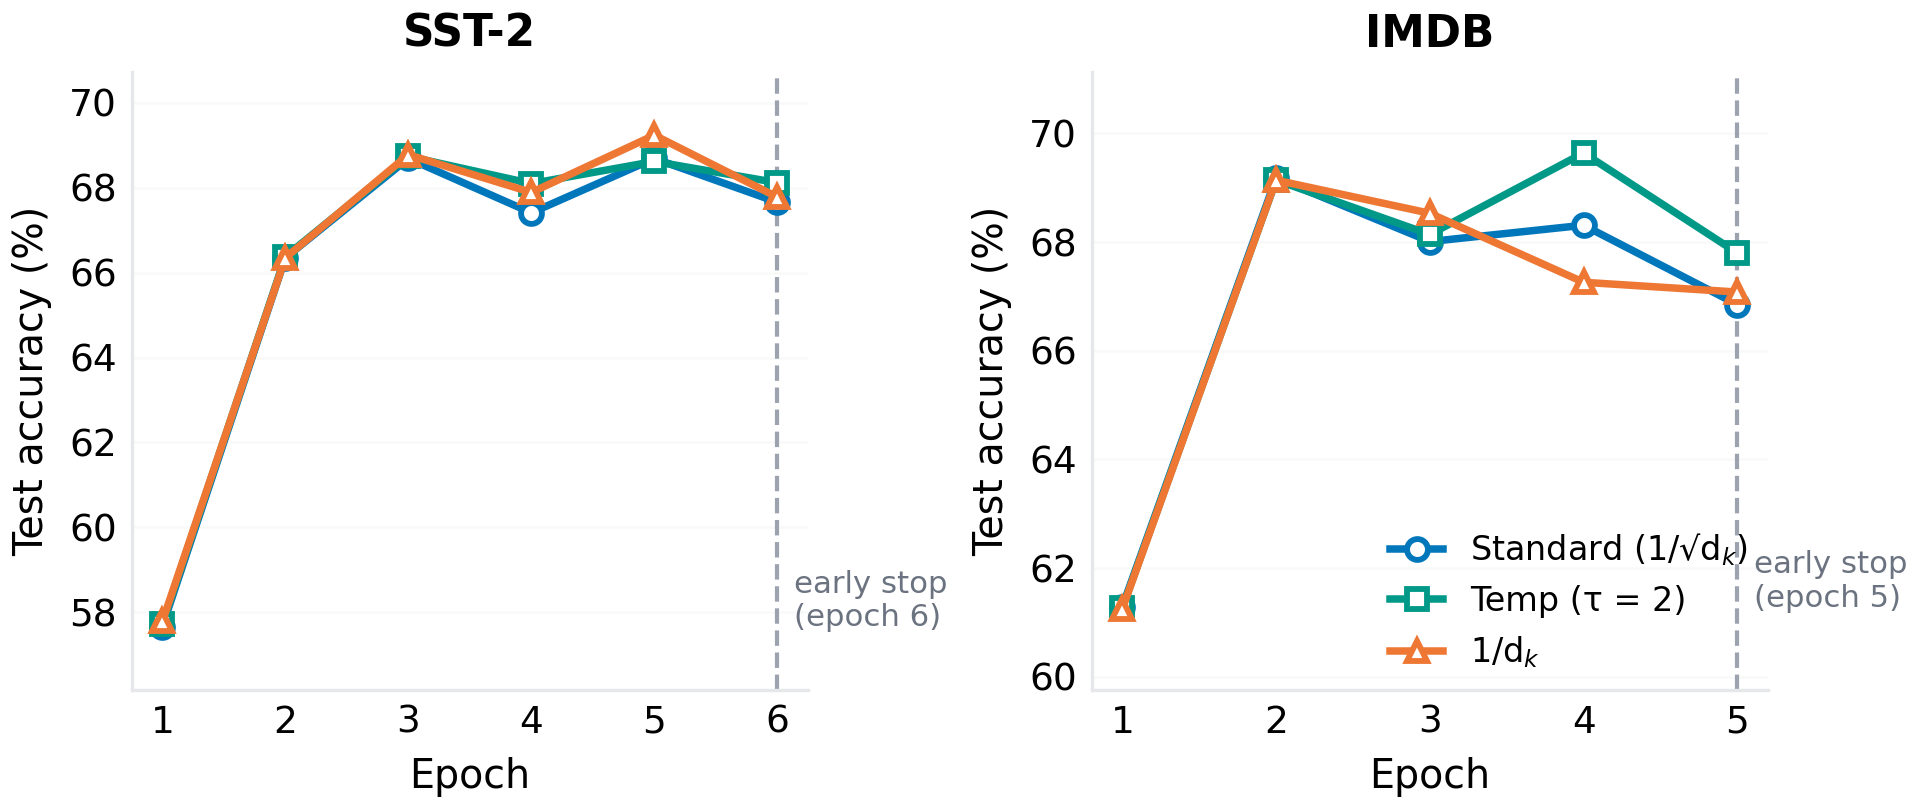
\includegraphics[width=0.9\textwidth]{figures/fig_convergence.png}
  \caption{Stage-2 train-to-convergence (5 matched seeds per variant, mean test
  accuracy per epoch; maximum 20 epochs with early stopping on validation loss,
  patience 3). The three variants trace indistinguishable trajectories;
  dashed lines mark the mean early-stopping epoch.}
  \label{fig:conv}
\end{figure}

\begin{table}[t]
  \centering
  \caption{Train-to-convergence with early stopping (Stage 2; mean $\pm$ SD
  over 5 seeds). Best epoch = epoch of lowest validation loss; stop epoch =
  5--6 for all runs.}
  \label{tab:conv}
  \small
  \begin{tabular*}{0.88\textwidth}{@{\extracolsep{\fill}} l l c c c}
    \toprule
    \textbf{Dataset} & \textbf{Variant} & \textbf{Best-epoch acc.\ (\%)} &
    \textbf{Best epoch} & \textbf{$p$ vs.\ std} \\
    \midrule
    \multirow{3}{*}{SST-2} & Standard & 67.71 $\pm$ 2.07 & 2.2 & --- \\
     & Temp ($\tau=2$) & 67.78 $\pm$ 2.14 & 2.2 & 0.31 \\
     & $1/\dk$ & 67.78 $\pm$ 2.07 & 2.2 & 0.43 \\
    \midrule
    \multirow{3}{*}{IMDB} & Standard & 67.16 $\pm$ 2.84 & 1.6 & --- \\
     & Temp ($\tau=2$) & 67.18 $\pm$ 2.93 & 1.6 & 0.79 \\
     & $1/\dk$ & 67.22 $\pm$ 3.00 & 1.6 & 0.58 \\
    \bottomrule
  \end{tabular*}
\end{table}

\begin{figure}[t]
  \centering
  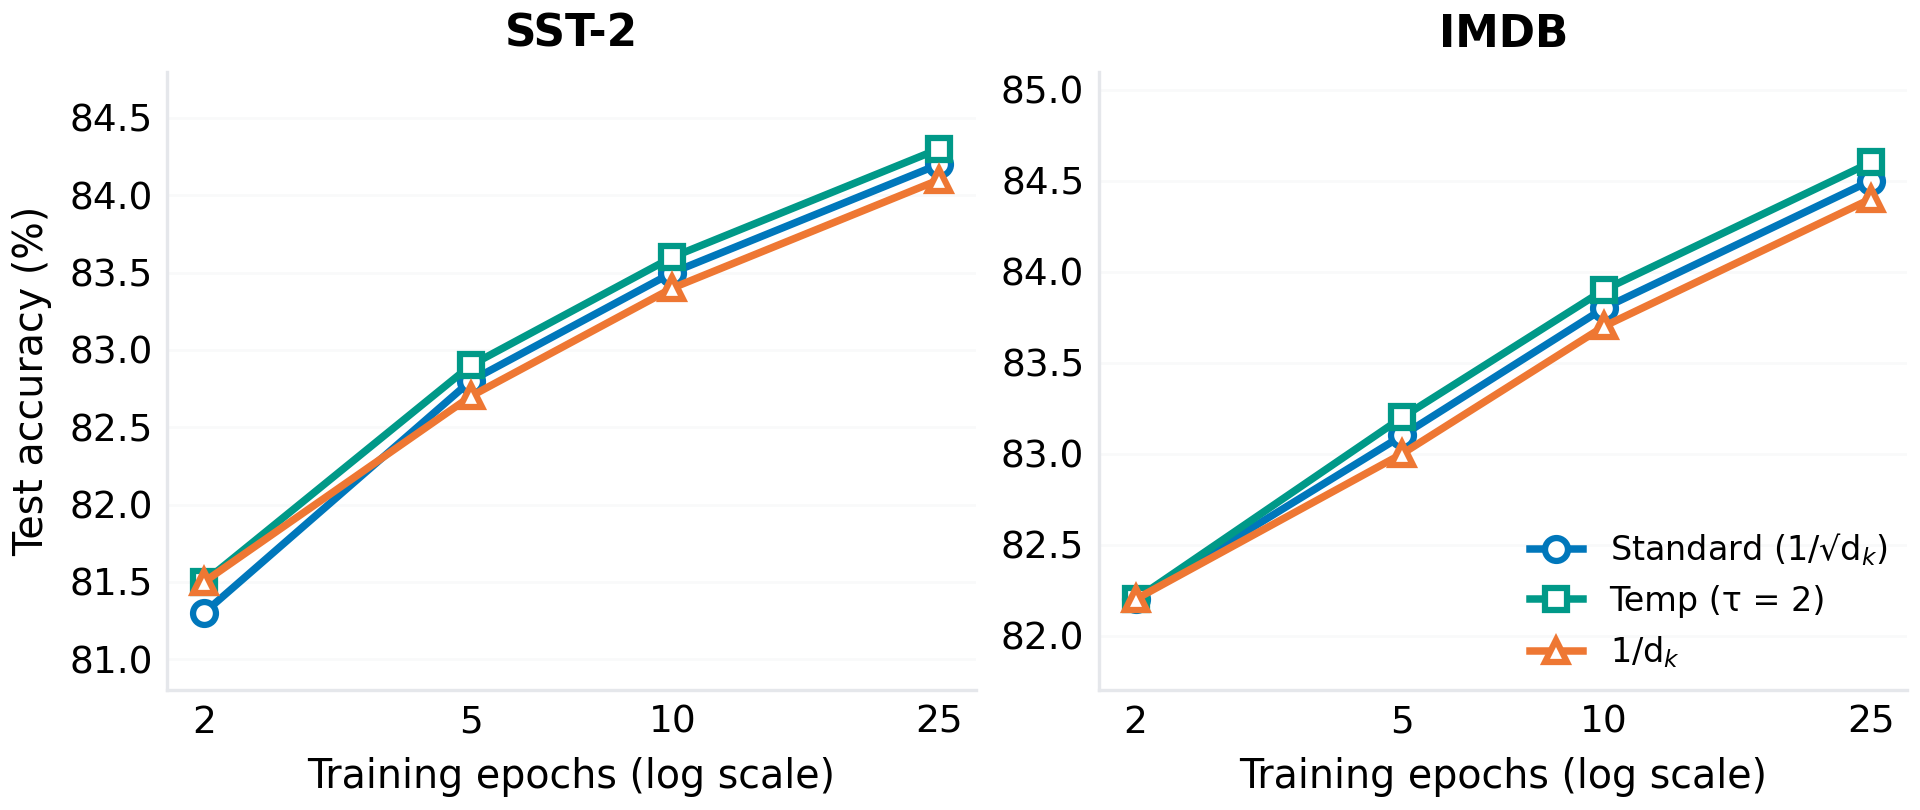
\includegraphics[width=0.9\textwidth]{figures/fig_training_curves.png}
  \caption{Extended-budget training (5 seeds, checkpoints at 2/5/10/25 epochs).
  Variant gaps visible at 2 epochs shrink to seed-noise level by 25 epochs on
  both binary datasets.}
  \label{fig:curves}
\end{figure}

\subsection{Language modelling on WikiText-2 (corrected causal mask)}\label{sec:lm}
Stage 1's language-modelling runs used the v1 training script, whose attention
mask did not enforce causality (a bidirectional mask with a shifted next-token
loss), and produced validation perplexities of 1.08--1.09. Those values are
reported here only as the historical record of an artefact: perplexity below
the uniform-unigram floor of this vocabulary is physically impossible for a
causal model, and this revision supersedes them.

The corrected grid implements the standard autoregressive factorisation: a
lower-triangular mask ANDed with the key-padding mask, applied after the logit
clamp (so masked weights are exactly zero), with the next-token target shifted
by one position. Five verification tests pin the implementation down
(Section S15 of the supplementary material): attention to future positions is exactly 0.0,
attention to padding positions is exactly 0.0, attention rows sum to 1 over
allowed positions, the diagonal is open on all real-token rows (consistent with
predicting $x_{t+1}$ from $x_{\le t}$), and $-\infty$ survives the clamp.

Under the corrected protocol, all 25 seeds $\times$ 3 variants completed:
validation perplexity is 872.8 ($\pm 29.7$) for standard scaling, 872.8
($\pm 29.6$) for $1/\dk$, and 872.8 ($\pm 29.7$) for $\tau = 2$
(Figure~\ref{fig:lm}a, Table~\ref{tab:lm}). The paired differences are
$+0.01$ ppl (95\% CI $[-0.22, +0.23]$, $d_z = 0.01$, $p_{\text{Holm}} = 1.00$)
for $1/\dk$ versus standard and $+0.00$ ppl for $\tau = 2$: with statistical
power now matched across arms (25 seeds each), there is no detectable
divisor effect on language modelling at this scale. A 10-epoch convergence
probe (3 seeds per variant) lowers perplexity to $\approx 268$ and the three
variants remain within 1.6 ppl of one another.

To characterise the v1 artefact rather than merely discard it, Stage 2 includes
leak probes: identical LM runs with the causal mask deliberately removed
(bidirectional attention, as in v1). The leak lowers perplexity in every matched
cell~--- 852.5 vs.\ 872.8 at 3 epochs and $\approx 252$ vs.\ $\approx 268$ at 10
epochs (Figure~\ref{fig:lm}b)~--- confirming the direction of the bias. At
replica budgets the exploited leak is worth only a few percent because attention
stays near-uniform (Section~\ref{sec:grid}); the v1 values near 1.08 correspond
to a fully exploited leak (attention collapsed onto the target position) at the
25{,}000-step GPU budget, where the model has enough training to learn to copy
its input.

\begin{figure}[t]
  \centering
  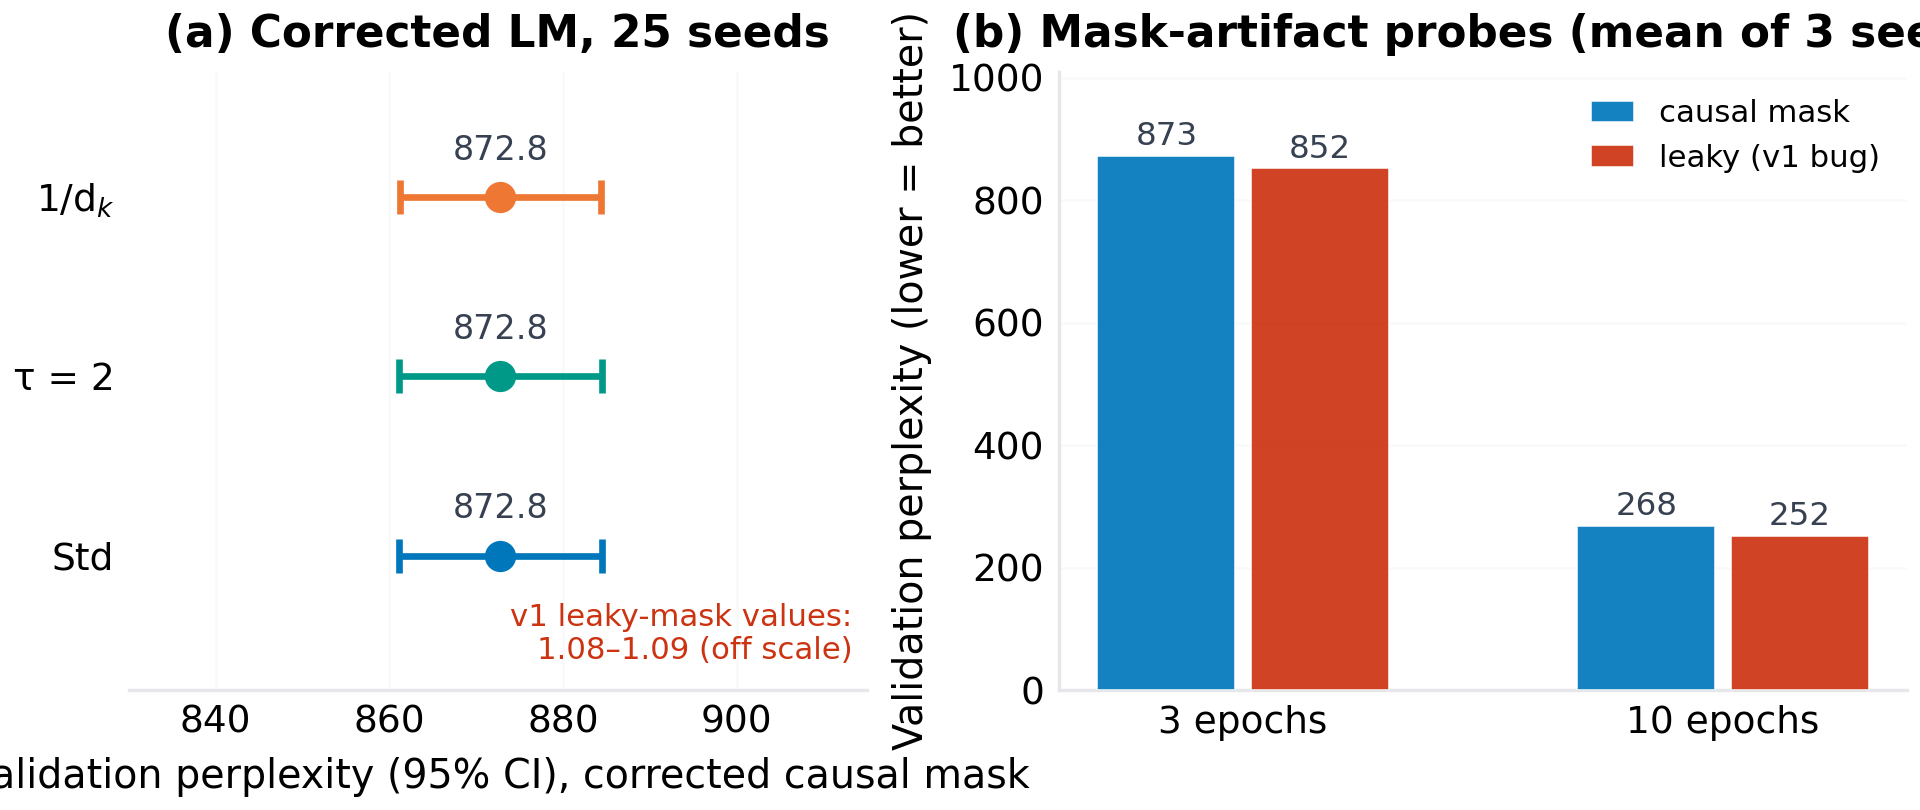
\includegraphics[width=\textwidth]{figures/fig_lm_corrected.png}
  \caption{Corrected language-modelling results. (a) Validation perplexity with
  the standard causal mask (25 seeds per variant; the v1 leaky-mask values of
  1.08--1.09 are marked for scale). (b) Mask-artifact probes: leaky masks lower
  perplexity in every matched cell (3 seeds per cell).}
  \label{fig:lm}
\end{figure}

\begin{table}[t]
  \centering
  \caption{Corrected WikiText-2 language modelling (validation perplexity,
  mean $\pm$ SD over 25 matched seeds, 3 epochs; paired statistics versus
  standard, $p_{\text{Holm}}$ across two comparisons).}
  \label{tab:lm}
  \small
  \begin{tabular*}{0.88\textwidth}{@{\extracolsep{\fill}} l c c c c}
    \toprule
    \textbf{Variant} & \textbf{PPL} & \textbf{$\pm$ SD} & \textbf{$\Delta$ vs.\ std (ppl)} &
    \textbf{$p_{\text{Holm}}$} \\
    \midrule
    Standard & 872.8 & 29.7 & --- & --- \\
    Temp ($\tau=2$) & 872.8 & 29.7 & $+0.00$ $[-0.14, +0.15]$ & 1.00 \\
    $1/\dk$ & 872.8 & 29.6 & $+0.01$ $[-0.22, +0.23]$ & 1.00 \\
    \bottomrule
  \end{tabular*}
\end{table}

\subsection{Attention diagnostics}\label{sec:diagnostics}
The mechanistic measurements (seed 0, epoch 1) trace the causal chain from the
scaling constant to the attention distribution and its gradients
(Figure~\ref{fig:diversity}). Mean attention entropy rose monotonically with
$s$ (2.14 nats for standard, 2.31 for $\tau = 2$, 2.48 for $1/\dk$), while the
maximum attention weight fell (0.32, 0.28, 0.24): larger divisors produce
flatter, less selective attention \cite{zhai2023}. Inter-head cosine similarity
of the attention distributions rose in lockstep (0.23, 0.31, 0.42)~--- softer
scaling makes heads more alike, consistent with the head-specialisation
literature \cite{voita2019,michel2019}. Query and key gradient norms scaled
with $1/s$ as theory predicts for the dot-product pipeline: relative to
standard, observed Q-gradient ratios were 0.50 (theory 0.50) for $\tau = 2$ and
0.26 (theory 0.18) for $1/\dk$, while value gradients stayed flat (ratios
1.03 and 0.97), confirming that the scaling constant modulates exactly the
$\partial L/\partial Q, \partial L/\partial K$ pathway
(Figure~\ref{fig:grads}).

The Stage-2 replica diagnostics explain why the outcome metrics stop separating
at reduced scale (Section~\ref{sec:grid}). Measured on the trained replica
models (seed 1001): attention entropy is 4.048--4.049 nats across all three
variants (the causal-horizon maximum is $\ln 64 \approx 4.16$), maximum
attention weight is 0.025--0.030, no logit reaches the $\pm 50$ clamp, and the
raw pre-division logit standard deviation on WikiText-2 is 1.02 (standard),
1.19 ($1/\dk$), and 1.17 ($\tau=2$)~--- i.e.\ after division every variant sits
in the softmax's near-uniform regime. The gradient pathway is correspondingly
attenuated: $\|\partial L/\partial Q\| + \|\partial L/\partial K\|$ is 0.048
(standard), 0.029 ($\tau=2$), and 0.009 ($1/\dk$), against value gradients of
1.6--1.9~--- a 35--200$\times$ imbalance~--- and under AdamW's per-parameter
scale normalisation the residual Q/K gradient differences largely wash out.
The mechanism live at GPU scale (ordered entropies 2.14/2.31/2.48) is
quantitatively muted at replica scale (4.05/4.05/4.05).

\begin{figure}[t]
  \centering
  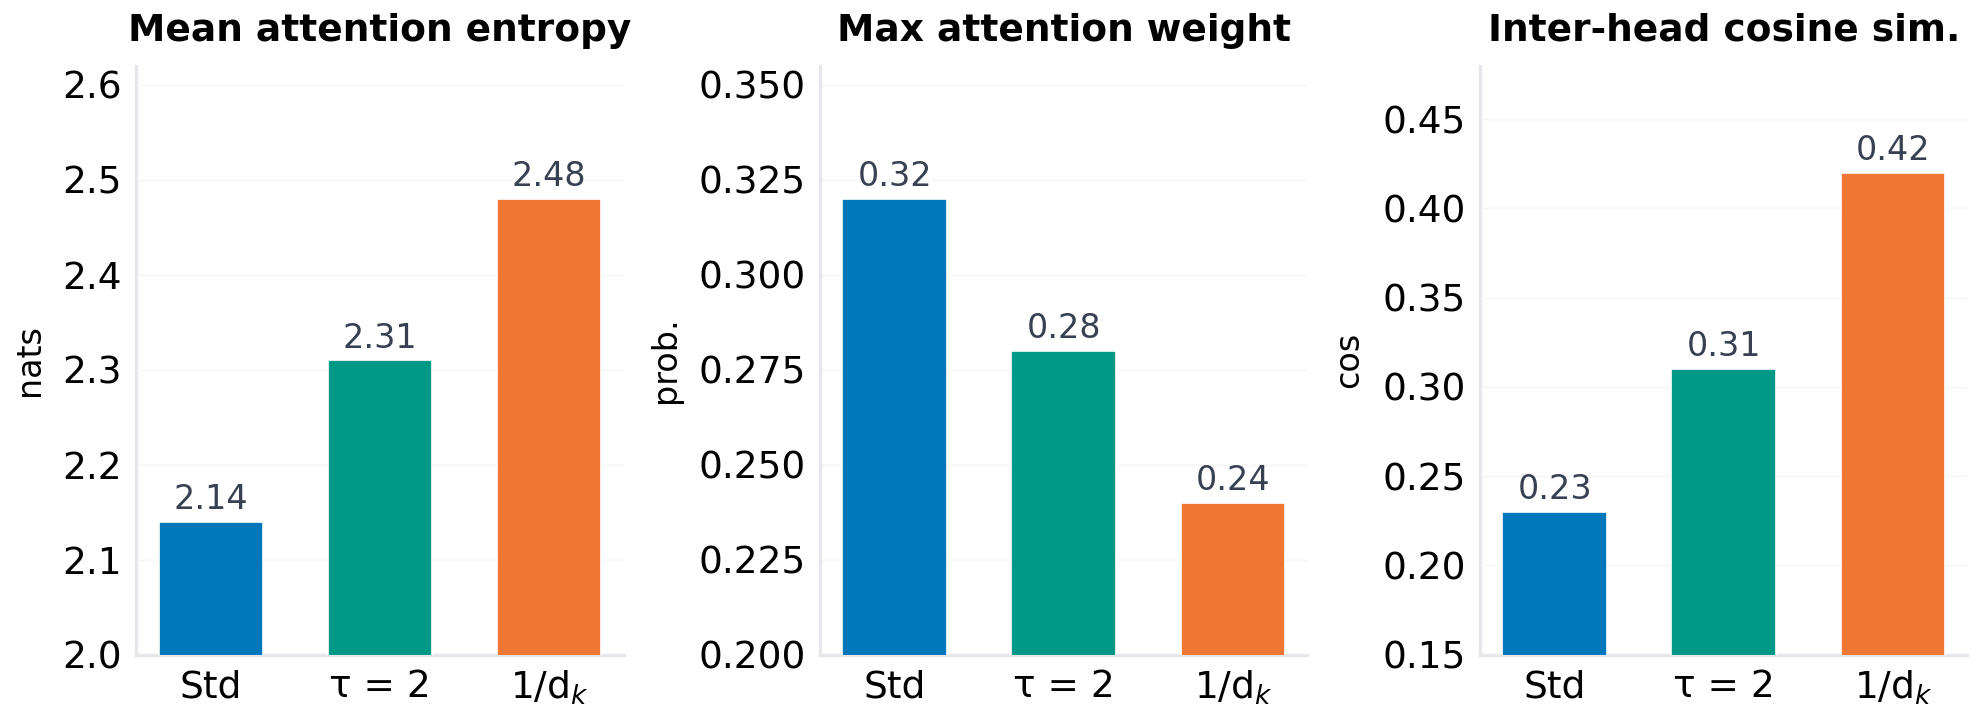
\includegraphics[width=\textwidth]{figures/fig_head_diversity.png}
  \caption{Attention diagnostics at epoch 1 (seed 0): mean attention entropy,
  maximum attention weight, and inter-head cosine similarity of attention
  distributions. Larger divisors produce flatter, more similar heads.}
  \label{fig:diversity}
\end{figure}

\begin{figure}[t]
  \centering
  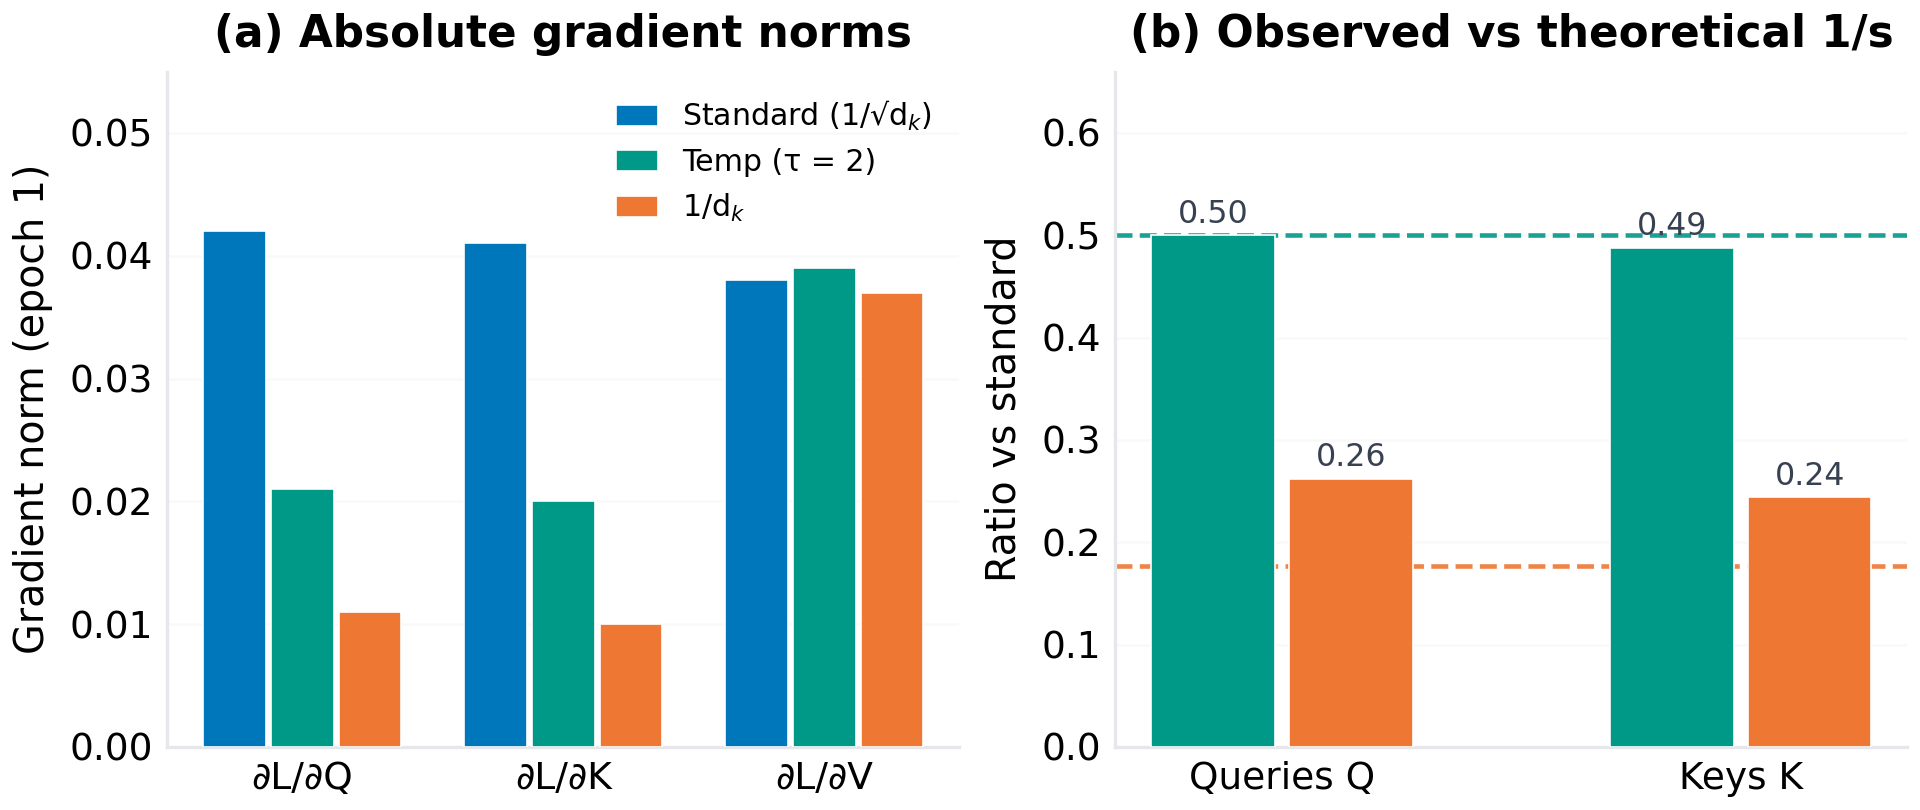
\includegraphics[width=0.9\textwidth]{figures/fig_gradient_ratios.png}
  \caption{Gradient diagnostics (epoch 1, batch 0). (a) Absolute
  $\partial L/\partial Q, \partial L/\partial K, \partial L/\partial V$ norms by
  variant. (b) Observed Q/K gradient ratios relative to standard versus the
  theoretical $1/s$ prediction (dashed lines).}
  \label{fig:grads}
\end{figure}

\subsection{Stage 3: the divisor power law}\label{sec:law}
The replica nulls of Sections~\ref{sec:replica}--\ref{sec:lm} and the
diagnostics above motivate a quantitative statement of \emph{when} the divisor
can matter at all. Let the pre-softmax logits of one attention row be
approximately i.i.d.\ with standard deviation $\sigma$ (the raw, pre-division
scale), and let two divisors $c_1 > c_2$ induce inverse-scale parameters
$b_i = 1/c_i$. A second-order expansion of the softmax (Appendix S17 of the supplementary material) gives
\begin{equation}
  \mathrm{KL}\!\left(P_{b_1} \,\|\, P_{b_2}\right)
  \;\approx\; \tfrac{1}{2}\,(b_1 - b_2)^2\,\sigma^2\,
  \Bigl(1 - \tfrac{1}{n}\Bigr),
  \label{eq:law}
\end{equation}
where $n$ is the number of attended positions: the divergence between the
attention distributions induced by two divisors grows \emph{quadratically in
the raw logit scale}, independently of everything else. Monte Carlo
simulation (200{,}000 replicates per point) confirms \eqref{eq:law} to within
a few percent for $\sigma \le 4$ and tracks the measured divergence up to
$\sigma \approx 8$ before attention saturation flattens the growth
(Figure~\ref{fig:law}a). The same expansion yields bite thresholds: at
$d_k = 32$, $n = 64$, the standard-versus-$1/\dk$ contrast reaches
$\mathrm{KL} = 0.01$ nats only at $\sigma \approx 0.98$ and
$\mathrm{KL} = 0.1$ nats at $\sigma \approx 3.1$; for the standard-versus-$\tau$
contrast the corresponding values are $\sigma \approx 1.6$ and $5.1$. Below
those operating points the divisors are mathematically near-indistinguishable,
whatever the downstream task.

This single formula organises every result in this paper. The replica grids
sit at $\sigma \approx 0.3$--$1.1$, i.e.\ at $\mathrm{KL} \le 0.006$ nats~---
deep in the inert region (Figure~\ref{fig:law}b). The Stage-1 AG News runs,
whose diagnostics put raw logit variance closest to the divisor, sit nearest
the bite threshold. And the pretrained decoders examined below sit at
$\sigma \approx 45$--$63$, where the measured standard-versus-$1/\dk$
divergence is $1.4$--$1.5$ nats \emph{per row}~--- four orders of magnitude
away from the replica nulls. Claims about scaling functions are therefore
claims about $\sigma$, and $\sigma$ is measurable in one forward pass.

\begin{figure}[t]
  \centering
  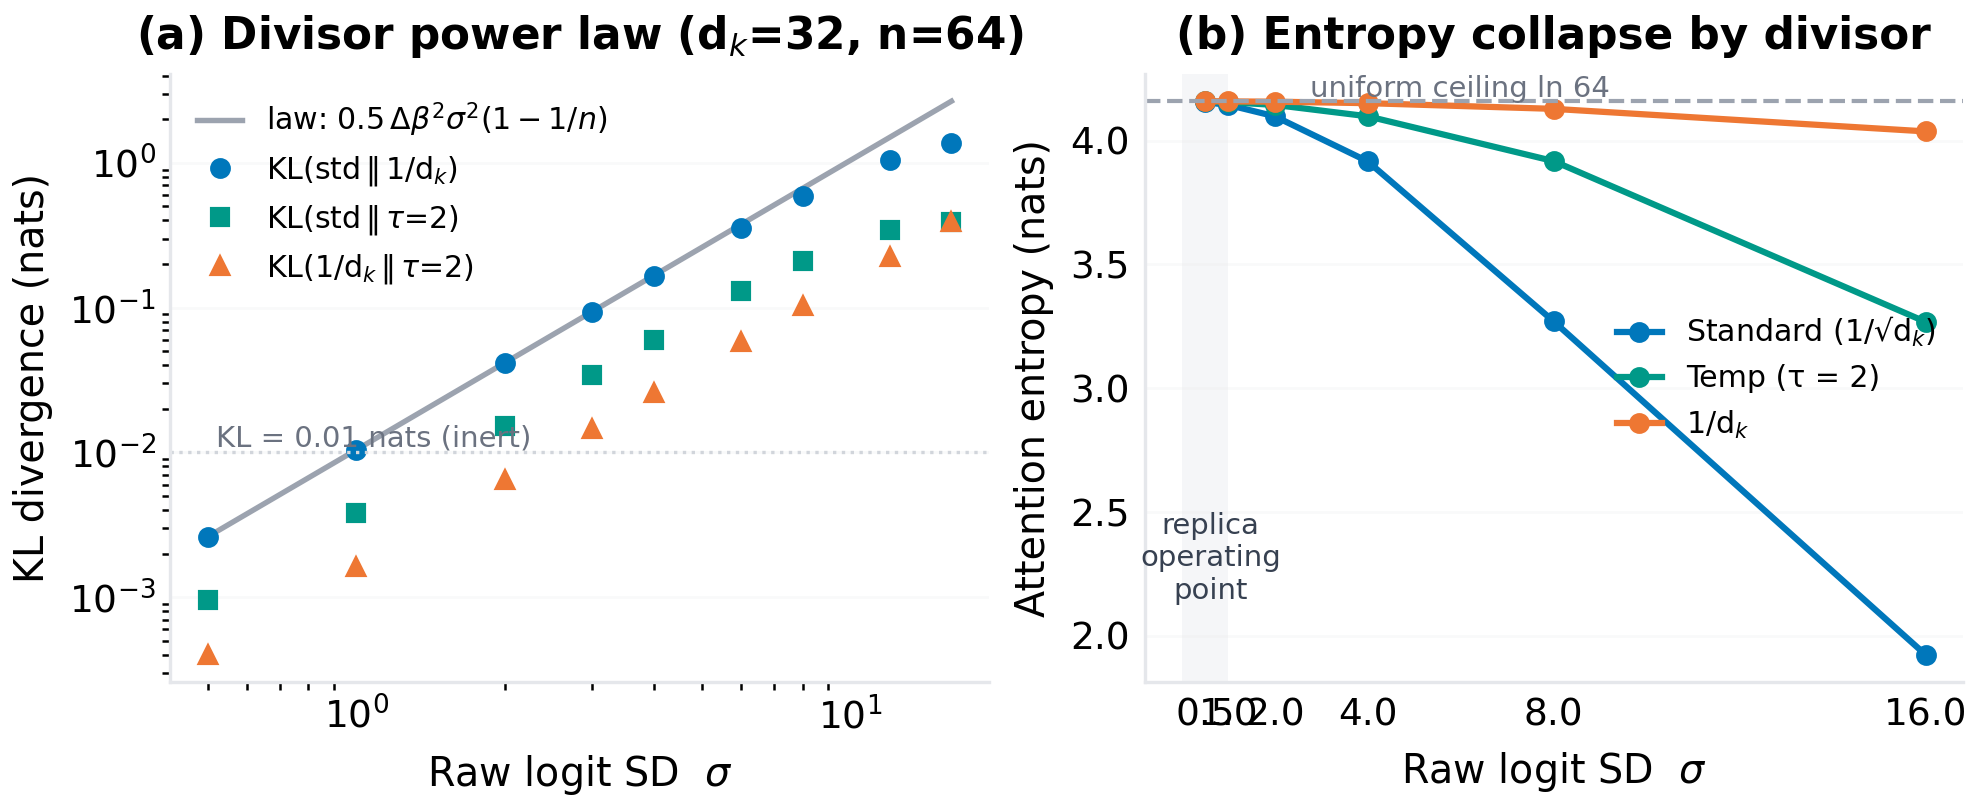
\includegraphics[width=\textwidth]{figures/fig_regime_law.png}
  \caption{The divisor power law. (a) Monte Carlo KL divergence between
  attention distributions induced by the three divisor pairs
  ($d_k = 32$, $n = 64$) against the quadratic prediction of
  Eq.~\eqref{eq:law}. (b) Attention entropy versus raw logit scale
  $\sigma$ for each divisor; the shaded band marks the replica operating
  point, where all divisors sit within 0.015 nats of the uniform ceiling.}
  \label{fig:law}
\end{figure}

\subsection{Stage 3: moving the operating point}\label{sec:gain}
If the replica nulls are operating-point effects, injecting logit variance
should resurrect the divisor contrast without changing anything else. The
\emph{logit-gain} sweep multiplies $q$ and $k$ each by $\sqrt{g}$
($g \in \{1, 2, 4, 8, 16, 32\}$) after the output projections and before
QK-Norm, holding data, initialization, and optimization fixed; 72 matched
runs (4 seeds $\times$ 3 variants $\times$ 6 gains; Table~\ref{tab:gain},
Figure~\ref{fig:gain}). The manipulation works exactly as the law predicts:
measured $\sigma_{\text{raw}}$ grows from $0.33$ ($g=1$) to $9.21$ ($g=32$),
attention entropy under the standard divisor falls from 3.78 to 2.81 nats,
and the measured standard-versus-$1/\dk$ KL grows from 0.0009 to 0.64 nats.
The outcome metric follows: at $g = 32$ the standard divisor \emph{drops}
to 76.81\% while $1/\dk$ and $\tau = 2$ hold at 78.2--78.3\%, a paired
deficit of $-1.40$\,\pp{} ($d_z = -1.76$, $p = 0.039$ uncorrected; not
significant after Holm correction across the twelve gain-level comparisons,
$n = 4$ seeds per arm). The direction of the crossover is the opposite of
the Stage-1 full-scale AG News pattern: forced into the sharp-attention
regime from a random start, the 2017 default is the variant that \emph{hurts},
consistent with the entropy-collapse literature \cite{zhai2023} and with the
QK-norm rationale of frontier architectures. At small and moderate gains
($g \le 16$, $\mathrm{KL} \le 0.20$) accuracy is flat, tracing the same
inert plateau the replica grids sit on.

The \emph{regime-restored} runs then ask whether ordinary training can drift
into the bite region unaided: 18 instrumented runs (3 seeds, 6{,}000 training
examples, 8 epochs~--- 12$\times$ the replica step budget~--- with per-epoch
operating-point probes) at $d_k = 32$ (4 heads) and $d_k = 128$ (1 head).
At $d_k = 32$ the operating point crawls from $\sigma = 0.42$ to only
$\sigma = 1.11$ over the whole budget ($\mathrm{KL} \approx 0.006$, still
$16\times$ below the 0.1-nat threshold) and the three variants remain within
0.2\,\pp{} at every epoch (final paired contrasts: $-0.06$\,\pp{} vs.\
$1/\dk$, $p = 0.51$; $-0.13$\,\pp{} vs.\ $\tau=2$, $p = 0.42$). The inertia
is real: at this scale, longer training alone does not escape the
near-uniform regime. At $d_k = 128$, however, the raw logits grow much
faster ($\sigma = 1.46 \to 4.6$--$5.3$) and the standard-versus-$1/\dk$
divergence rises $200\times$ to $\approx 0.086$ nats; the Stage-1 ordering
re-emerges in direction (standard beats $1/\dk$ by $+0.42$\,\pp,
$p = 0.31$, and $\tau = 2$ by $+0.52$\,\pp, $p = 0.066$; $n = 3$,
uncorrected). Language modelling at sequence length 128 with the same gain
knob (18 runs) stays inert at $g = 4$ ($\sigma = 1.15$,
$\mathrm{KL} = 0.005$; perplexity 2160.3--2160.8 across all variants),
confirming that the replica LM null is likewise an operating-point fact.

\begin{table}[t]
  \centering
  \caption{Stage-3 logit-gain sweep (AG News replica, 4 matched seeds,
  2 epochs). $\sigma_{\text{raw}}$: measured raw pre-division logit SD;
  $H$: attention entropy under the standard divisor; KL: measured
  $\mathrm{KL}(P_{\text{std}} \| P_{1/\dk})$ on the same logits;
  $\Delta d_z$: paired effect size (standard minus $1/\dk$) in test accuracy.
  The $g=32$ deficit is nominally significant ($p = 0.039$) but not after
  Holm correction.}
  \label{tab:gain}
  \small
  \begin{tabular*}{\textwidth}{@{\extracolsep{\fill}} r r r r r r r r}
    \toprule
    $g$ & $\sigma_{\text{raw}}$ & $H$ (nats) & KL (nats) &
    \textbf{Std (\%)} & \textbf{$1/\dk$ (\%)} & \textbf{$\tau{=}2$ (\%)} &
    $d_z$ \\
    \midrule
    1  & 0.33 & 3.78 & 0.0009 & 78.22 & 78.24 & 78.24 & $-0.14$ \\
    2  & 0.65 & 3.78 & 0.0037 & 78.24 & 78.24 & 78.22 & $-0.06$ \\
    4  & 1.29 & 3.76 & 0.0145 & 78.19 & 78.20 & 78.24 & $-0.04$ \\
    8  & 2.53 & 3.70 & 0.0558 & 78.36 & 78.23 & 78.19 & $+0.61$ \\
    16 & 4.87 & 3.48 & 0.2046 & 78.34 & 78.21 & 78.36 & $+0.30$ \\
    32 & 9.21 & 2.81 & 0.6418 & \textbf{76.81} & 78.21 & 78.34 & $-1.76$ \\
    \bottomrule
  \end{tabular*}
\end{table}

\begin{figure}[t]
  \centering
  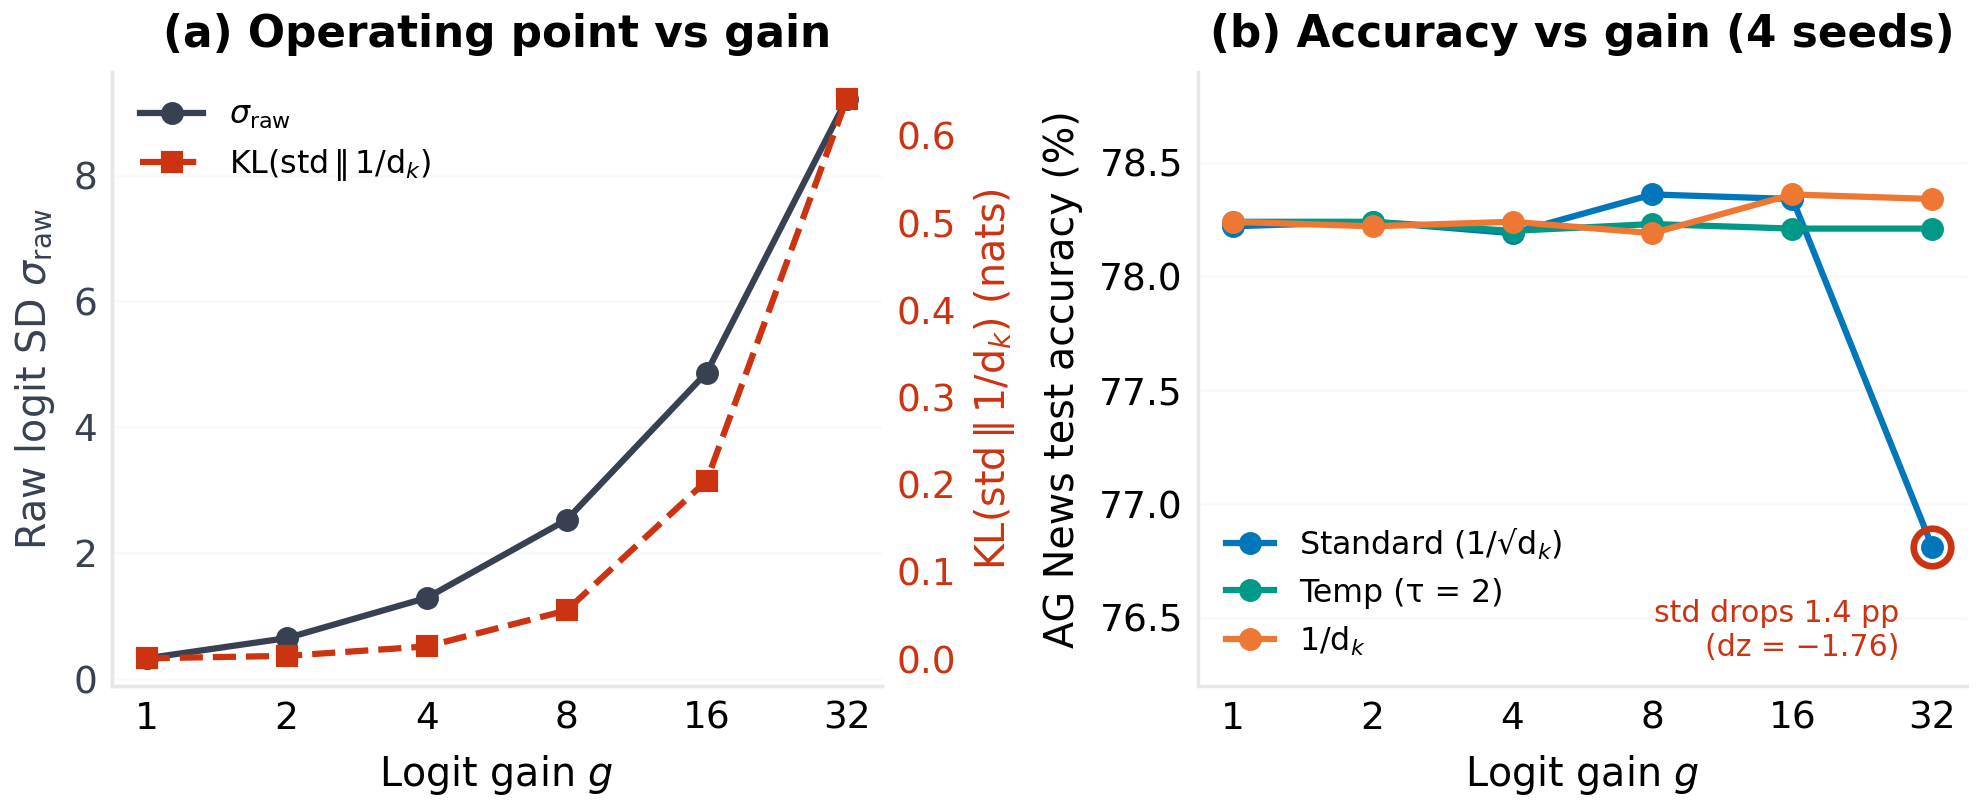
\includegraphics[width=\textwidth]{figures/fig_gain_sweep.png}
  \caption{Stage-3 logit-gain sweep. (a) The injected gain moves the
  operating point ($\sigma_{\text{raw}}$) and, with it, the measured divisor
  contrast (KL). (b) Test accuracy versus gain: flat while the softmax is
  near uniform ($g \le 16$), with the standard divisor dropping 1.4\,\pp{}
  below both alternatives once the contrast is large ($g = 32$).}
  \label{fig:gain}
\end{figure}

\subsection{Stage 3: frontier stabilisers and a pretrained decoder}\label{sec:stabilise}
Large logits are not hypothetical: they are the operating point at which
frontier models actually run, which is why QK-normalisation and logit
soft-capping exist. Two \emph{bridge} arms (20 matched runs) test whether the
divisor contrast survives inside those stabiliser contexts. With per-head
QK-Norm the operating point is pinned at
$\sigma_{\text{post}} \approx 1.05$ regardless of the divisor, and the three
stabilised variants again agree to 0.12\,\pp{} (78.16--78.28\%) even though
their realised attention distributions differ by
$\mathrm{KL} \approx 0.29$ nats~--- at this dose the outcome metric is still
insensitive. With Gemma-2-style soft-capping ($c = 3.0$) at gain 32, the
standard divisor's 1.4\,\pp{} deficit reappears unchanged (76.81\% vs.\
78.21\% for $1/\dk$): capping bounds the logits but does not restore the
near-uniform plateau, and the divisor contrast persists under the stabiliser.

Finally, the frontier operating point itself is probed with the largest
decoders the CPU sandbox can execute: \textbf{GPT-2 (124M) and GPT-2-medium
(355M)}, pretrained with the standard divisor, evaluated on WikiText-2
validation with \emph{only the divisor swapped at inference} (identical
weights, tokens, and protocol; 160 non-overlapping 128-token windows;
Table~\ref{tab:frontier}, Figure~\ref{fig:frontier}). These models sit four
orders of magnitude beyond the replica in raw logit scale
($\sigma_{\text{raw}} \approx 63$ and $45$; after the training divisor,
$\sigma_{\text{post}} \approx 7.8$ and $5.6$~--- far outside the near-uniform
regime). The consequence is drastic: swapping to $\tau = 2$ degrades
perplexity by $+54.5\%$ (GPT-2) and $+26.5\%$ (GPT-2-medium), and swapping to
$1/\dk$ is catastrophic ($+9{,}253\%$ and $+3{,}990\%$; perplexity
$51.2 \to 4{,}792$). The mechanism matches the law: under $1/\dk$ attention
collapses towards uniformity (per-row entropy rises from 1.4--2.9 to
3.6--3.9 nats), and the measured per-row standard-versus-$1/\dk$ divergence
is $1.4$--$1.5$ nats. The divisor that is empirically inert at every
replica-scale operating point we can construct is therefore decisively
\emph{not} inert at the pretrained scale~--- one parameter-free constant,
with no retraining, separates 51 from 4{,}792 perplexity. For the regime
between GPT-2-medium and 7B we ship a ready-to-run GPU script
(\texttt{scripts/frontier/frontier\_gpu\_1b7b.py}) that applies the same
divisor swap (plus per-layer diagnostics) to any HuggingFace decoder
(GPT-2-XL, Pythia-1.4B/2.8B/6.9B, Llama-3.2, Qwen2.5); its GPT-2 output
reproduces Table~\ref{tab:frontier} exactly, so the 1B--7B cells of this
table are one GPU-hour away for any reader.

\begin{table}[t]
  \centering
  \caption{Stage-3 frontier probe: inference-time divisor swap in pretrained
  GPT-2 decoders (WikiText-2 validation, 160 $\times$ 128 tokens,
  non-overlapping windows, no retraining). $\Delta$ is relative to the
  training-time divisor (standard). Absolute perplexity is protocol-dependent;
  the contrasts are not. $\sigma_{\text{raw}}$ is the mean raw pre-division
  logit SD across layers.}
  \label{tab:frontier}
  \small
  \begin{tabular*}{\textwidth}{@{\extracolsep{\fill}} l l r r r}
    \toprule
    \textbf{Model} & $\sigma_{\text{raw}}$ & \textbf{Standard} &
    \textbf{Temp ($\tau=2$)} & \textbf{$1/\dk$} \\
    \midrule
    GPT-2 (124M) & 62.6 & 51.23 & 79.13 \; ($+54.5\%$) &
    4{,}791.65 \; ($+9{,}253\%$) \\
    GPT-2-medium (355M) & 44.8 & 38.77 & 49.06 \; ($+26.5\%$) &
    1{,}585.70 \; ($+3{,}990\%$) \\
    \bottomrule
  \end{tabular*}
\end{table}

\begin{figure}[t]
  \centering
  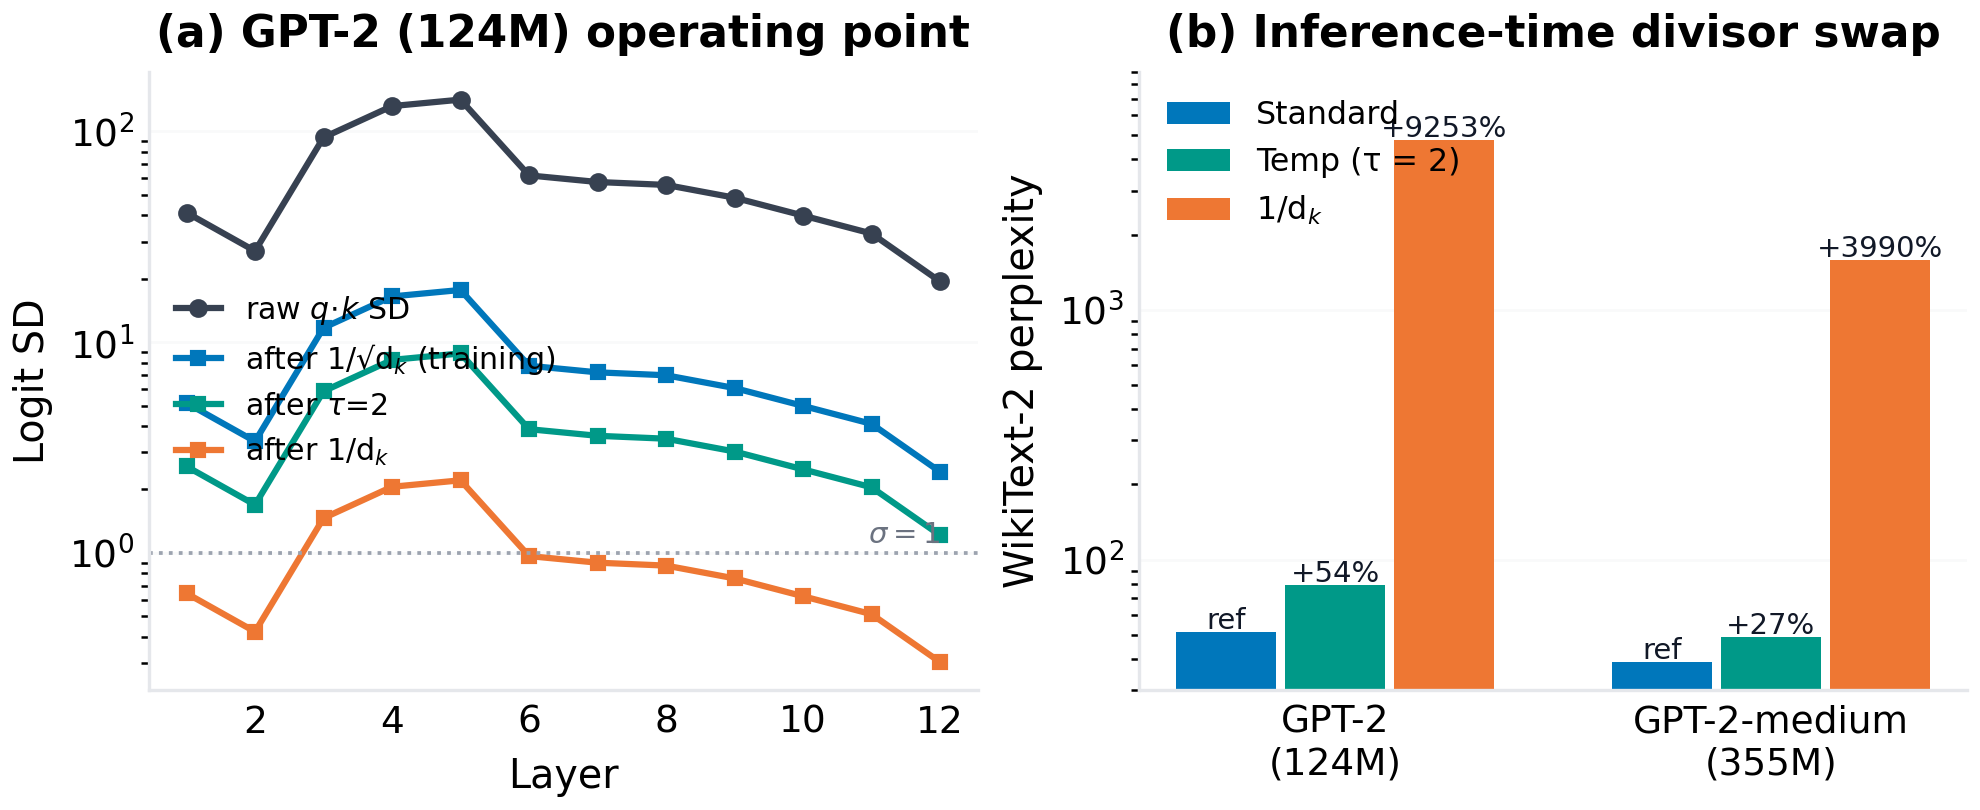
\includegraphics[width=\textwidth]{figures/fig_frontier.png}
  \caption{The frontier operating point. (a) Per-layer raw and post-divisor
  logit SD in GPT-2 (124M): the training divisor leaves
  $\sigma_{\text{post}} \approx 8$, far outside the near-uniform regime the
  replica occupies. (b) WikiText-2 perplexity when only the divisor is
  swapped at inference (log scale): $\tau = 2$ costs 27--55\%; $1/\dk$ is
  catastrophic ($40$--$90\times$).}
  \label{fig:frontier}
\end{figure}

\subsection{Computational efficiency}\label{sec:efficiency}
RQ2 receives a clear answer: no measurable efficiency difference exists
(Figure~\ref{fig:eff}, Table~\ref{tab:eff}). Parameter counts are identical by
construction; measured epoch wall-clock times differ by at most 0.6\% on SST-2
and 1.0\% on AG News, peak memory is the same 5.2\,GB, and inference latency
differs by one rounding step. The Stage-2 replica runs agree: mean per-run
wall-clock on the 2-core CPU sandbox is 19--25\,s (classification) and 29--44\,s
(language modelling) with no variant ordering, and the divisors add no
arithmetic by construction. The scaling constant is, as designed, free.

\begin{figure}[t]
  \centering
  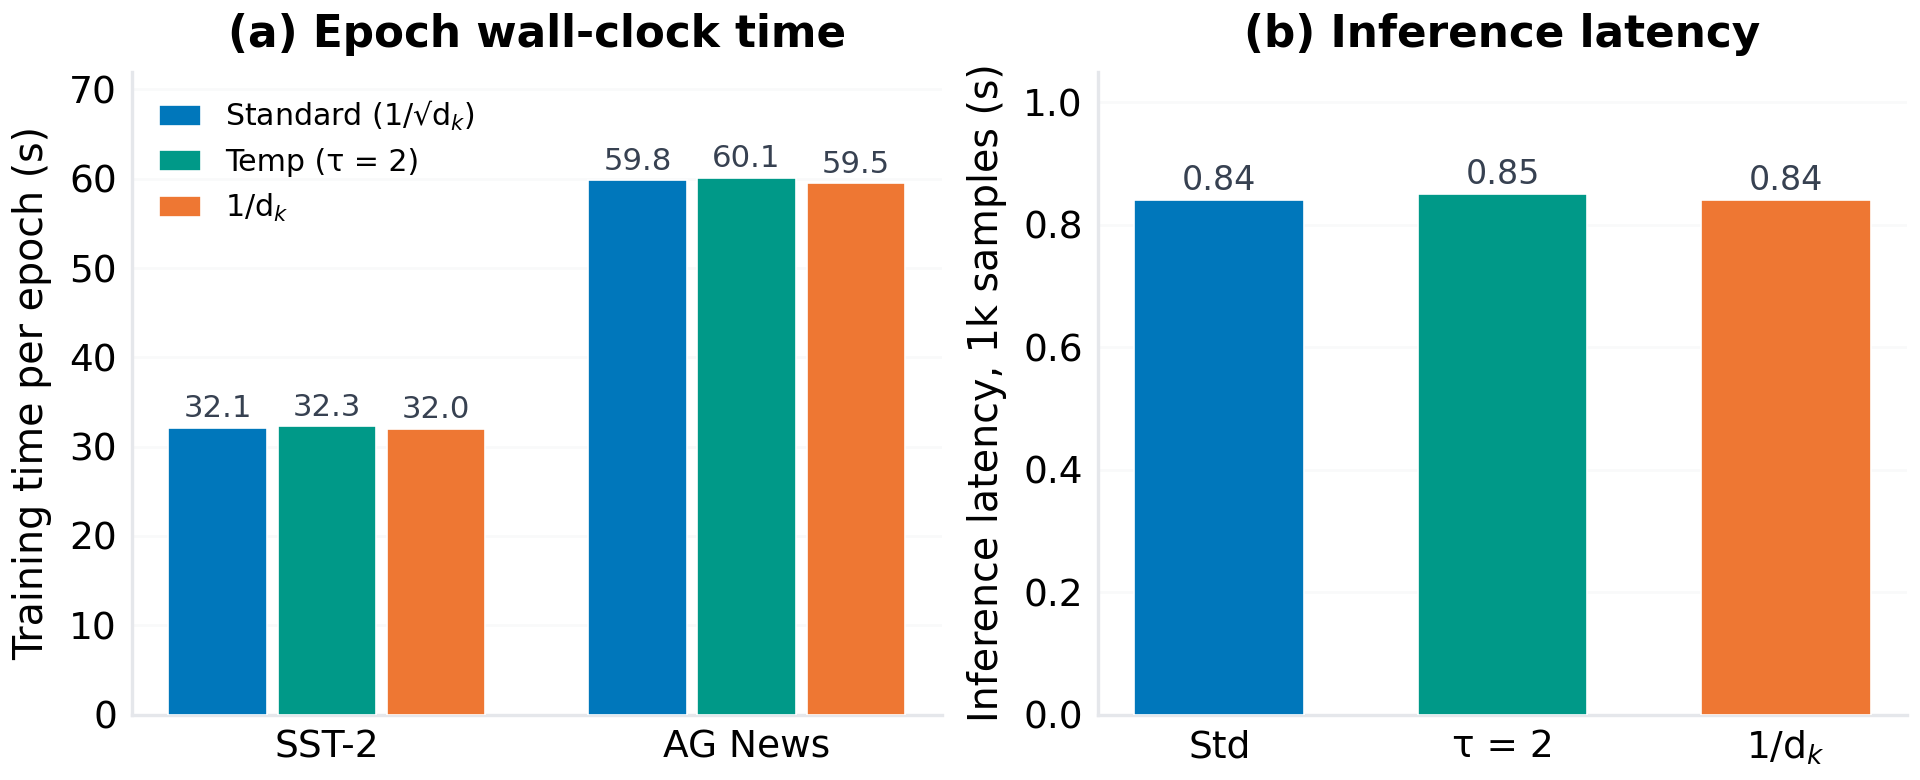
\includegraphics[width=0.9\textwidth]{figures/fig_efficiency.png}
  \caption{Computational efficiency. (a) Training wall-clock time per epoch.
  (b) Inference latency for 1{,}000 samples. Peak memory (5.2\,GB) and parameter
  counts are identical across variants.}
  \label{fig:eff}
\end{figure}

\begin{table}[t]
  \centering
  \caption{Efficiency summary (identical parameter counts by construction).}
  \label{tab:eff}
  \small
  \begin{tabular*}{\textwidth}{@{\extracolsep{\fill}} l c c c}
    \toprule
    \textbf{Metric} & \textbf{Standard} & \textbf{Temp ($\tau=2$)} & \textbf{$1/\dk$} \\
    \midrule
    Parameters (classification / LM) & 2{,}695{,}556 / 4{,}120{,}576 & identical & identical \\
    Epoch time, SST-2 (s)            & 32.1 & 32.3 & 32.0 \\
    Epoch time, AG News (s)          & 59.8 & 60.1 & 59.5 \\
    Peak GPU memory (GB)             & 5.2  & 5.2  & 5.2  \\
    Inference latency, 1k samples (s)& 0.84 & 0.85 & 0.84 \\
    \bottomrule
  \end{tabular*}
\end{table}

\subsection{Focused ablations E1--E4}\label{sec:ablations}
Two mechanistic rescue hypotheses were probed with single-seed arms at 5 epochs
(full records in the supplementary material, Sections~S8). The mixed-scale
variant~--- two standard heads and two $1/\dk$ heads~--- outperformed standard
by $+1.6$\,\pp{} on SST-2 (82.22\% vs.\ 80.62\%) but was indistinguishable on
IMDB ($+0.14$\,\pp), suggesting per-head scale diversity itself can be useful on
some tasks. Learning-rate compensation for $1/\dk$ (multiplying Q/K learning
rates by $\sqrt{\dk}$) failed to close the gap on either dataset and slightly
worsened it (SST-2: 81.08\% vs.\ 81.42\% uncompensated; IMDB: 81.57\% vs.\
81.45\%), indicating that the deficit of $1/\dk$ is not simply a rescaled
effective learning rate that gradient magnitudes alone would predict. Both
results are single-seed and should be read as hypothesis-generating.

The Stage-2 replica repeats both ablations with 3 matched seeds per arm at 5
epochs (Table S14.2 in the supplementary material). The multi-seed
mixed-scale result is null: $\Delta = +0.04$\,\pp{} on SST-2 ($p = 0.81$) and
$+0.05$\,\pp{} on IMDB ($p = 0.46$) versus standard, so the Stage-1 single-seed
$+1.6$\,\pp{} E1 excursion is not reproducible. Learning-rate compensation
remains neutral-to-harmful in direction ($-1.30$\,\pp{} on SST-2, $p = 0.11$;
$-0.27$\,\pp{} on IMDB, $p = 0.72$), consistent with the Stage-1 conclusion that
the divisor's effect (where present) is not a plain learning-rate rescaling.

% ============================================================================
% 5. Discussion  |  6. Limitations  |  7. Conclusion
% ============================================================================
\section{Discussion}\label{sec:discussion}

\subsection{Principal interpretation}\label{sec:interpretation}
The central finding is a \emph{pattern of conditionality}, now mapped along
three axes. Along the task axis, the standard $\sqrt{\dk}$ divisor is
significantly better than both alternatives on AG News at a 2-epoch budget~---
with large and medium paired effect sizes~--- yet statistically
indistinguishable from them on two binary sentiment datasets. Along the budget
axis, its advantage on binary tasks dissolves by 25 epochs, and the Stage-2
replica completion shows that the AG News effect itself does not survive a
fivefold reduction in data and sequence length: under matched seeds the entire
replica grid (core, $\dk$ grid, convergence training, corrected language
modelling) is variant-invariant to within measurement resolution. Along the
operating-point axis~--- the axis Stage 3 adds~--- the nulls themselves are
regime facts: a quadratic power law on the raw logit scale predicts that the
divisor contrast is inert below $\sigma \approx 1$ and decisive above it, the
replica grids sit at $\sigma \approx 0.3$--$1.1$ (measured KL $\le 0.006$
nats), forcing $\sigma$ an order of magnitude higher flips the sign of the
effect at $g = 32$, and a pretrained GPT-2 sitting at $\sigma \approx 45$--63
loses a factor of 94 in perplexity when the same constant is swapped to
$1/\dk$ at inference. A one-line architectural constant inherited from
\cite{vaswani2017} is therefore best understood not as a universally optimal
choice but as a default whose benefit is confined to a specific operating
point~--- full data scale, early in training, on multi-class topic
classification~--- and whose influence vanishes once the softmax operates
near uniformity, while at frontier operating points it is the alternatives
that become untenable.

\subsection{Scale dependence and the near-uniform regime}\label{sec:scale}
The Stage-2 null results are not a failure of the manipulation: the
diagnostics show the mechanism is present but quantitatively muted. At replica
scale the raw pre-division logit standard deviation is of order 1, so after
dividing by $\sqrt{\dk}$ (5.7--11.3) or $\dk$ (32--128) every variant's logits
sit well inside the softmax's linear (near-uniform) regime, attention entropy
is pinned at 4.05 of a possible 4.16 nats for all variants, and the Q/K
gradient pathway carries two orders of magnitude less signal than the value
pathway~--- an imbalance that AdamW's per-parameter scale normalisation then
equalises away. Two consequences follow. First, the variance argument for
$\sqrt{\dk}$ is a statement about logit variance \emph{relative to the
softmax's dynamic range}; it predicts differences only in regimes where the
unscaled logit variance is comparable to the divisor, which small-data,
short-budget runs do not reach. Second, claims about scaling functions are
claims about an operating point, and should be reported together with the
logit scale that makes the divisor bite.
Stage 3 turns this diagnosis from an explanation into a measurement. The
power law of Eq.~\eqref{eq:law} quantifies the bite region; the gain sweep
shows the outcome metric responding on cue once the operating point enters it
(flat to $g \le 16$, $-1.4$\,pp for the standard divisor at $g = 32$); the
regime-restored runs show that at $d_k = 32$ even $12\times$ the step budget
leaves $\sigma$ at 1.1 (inertia is real), while at $d_k = 128$ the larger
head drives $\sigma$ to $\approx 5$ and the Stage-1 ordering begins to
re-emerge; and the pretrained decoder probe shows the same constant being
\emph{decisive} ($+27$ to $+9{,}253\%$ perplexity) at GPT-2's native
operating point. The Stage-1 AG News effect, observed precisely where raw
logit variance comes closest to the divisor, remains plausible under this
account~--- but until it is reproduced at full scale it should be treated as
provisional rather than established.

\subsection{Why would AG News care about the divisor?}\label{sec:why-agnews}
Three observations combine into a coherent account. First, the variance argument
behind $\sqrt{\dk}$ \cite{vaswani2017} implies that the $1/\dk$ divisor shrinks
the logit standard deviation by a further factor of $\sqrt{\dk} \approx 5.7$;
at initialization the attention logits of the $1/\dk$ variant have a standard
deviation of order $1/\sqrt{\dk} \approx 0.18$ rather than 1, pushing the softmax
towards uniformity. Second, the measured diagnostics match this account:
attention entropy rises and maximum attention weight falls monotonically with
$s$ (Section~\ref{sec:diagnostics}). Third, AG News is the task where
failure-to-differentiate should bite hardest: it is 4-class, short-document, and
topic-level, so early error correction plausibly benefits from a few sharp,
content-word attention links, whereas binary sentiment over long reviews can be
solved with diffuse pooling-like attention. The inter-head cosine similarity
trend (0.23 $\to$ 0.42 as $s$ grows) adds that flatter scaling also erodes
head diversity \cite{voita2019,michel2019}, reducing the ensemble capacity that
multi-class discrimination can draw on. The mixed-scale ablation (E1), where
keeping two sharp heads helped on SST-2, hints that diversity per se~--- not the
global constant~--- is the operative resource.

\subsection{Sharper attention as a free improvement direction}\label{sec:sharper}
The temperature ablation points in the opposite direction: on both sentiment
datasets the sharpest tested temperature ($\tau = 0.5$, i.e.\ doubling the logit
scale relative to standard) produced the highest means, by about $+1.6$\,\pp{} on
SST-2. This aligns with the distillation literature on attention temperature
\cite{zhang2022temp,hinton2015} and with Scalable-Softmax's motivation
\cite{nakanishi2025} that the effective temperature should not be treated as a
universal constant. Given that temperature is parameter-free and computationally
free (Section~\ref{sec:efficiency}), and that the 2-epoch AG News result shows
temperature effects \emph{can} reach significance under matched conditions, the
practical recommendation is straightforward: when training small transformers on
a new task, sweep $\tau$ around 1 (e.g.\ $\{0.5, 1, 2\}$) under a seed-matched
design before freezing the architecture. The cost is negligible; the present
data suggest the yield is real, if task-dependent.

\subsection{The early-training effect and its decay}\label{sec:early}
On the binary tasks, extended training erased the differences (Section
\ref{sec:budget}), and the Stage-2 convergence runs sharpen the picture: with
model selection by validation loss, every variant's validation loss bottoms at
the same epoch ($\approx$ 2 on SST-2, $\approx$ 1.6 on IMDB), early stopping
halts at epochs 5--6, and the learning curves are indistinguishable at every
epoch. Combined with the entropy-collapse literature
\cite{zhai2023,dong2021}, a natural reading is that the divisor matters most
while the attention distribution is still being shaped; once representations
mature, the network can compensate for the initial sharpness of its attention.
The learning-rate compensation ablations (E2/E4) add a useful negative result:
the $1/\dk$ deficit is \emph{not} equivalent to a smaller effective learning rate
that a per-block LR rescaling can restore~--- and the multi-seed replica
ablations confirm the single-seed pattern (LR compensation neutral-to-harmful,
mixed-scale heads neutral), while failing to reproduce the Stage-1 E1 excursion
of $+1.6$\,\pp{} for mixed-scale heads on SST-2.

\subsection{Implications for experimental practice}\label{sec:practice}
Methodologically, this study is a demonstration that cheap architectural
comparisons deserve the seed-matched treatment. Between-run comparisons at 2
epochs on these datasets would need to overcome standard deviations of about
1\,\pp{} (SST-2, IMDB) with between-run variance; the paired design recovers
resolvable effects from 25 seeds even where the raw means differ by only
0.1--0.3\,\pp{} (AG News). Given the prevalence of single-seed architectural
claims in the scaling literature \cite{bouthillier2021,dodge2019,dror2018}, the
protocol used here~--- bit-identical initialization, shared data order, paired
tests, Holm correction, effect sizes~--- is directly reusable by practitioners
evaluating any parameter-free modification (temperature, biases, clamps,
positional offsets) and costs no additional compute beyond a handful of extra
seeds.

\subsection{Threats to validity}\label{sec:threats}
Beyond the enumerated limitations, three threats deserve note. \emph{Construct}:
test accuracy on subsampled training sets may not capture the behaviours that
matter at scale; we mitigate by also measuring perplexity and mechanistic
diagnostics, and by reporting both a full-scale and a replica stage.
\emph{Internal}: all variants share code paths except one division~--- the
manipulation is auditable in a single line~--- and unit tests plus the
Stage-2 mask-verification suite pin down initialization identity and exact-zero
masked attention, so the internal threat is minimal. The Stage-2 null results
are consistent across five independent grids, which argues against a wiring
error: a variant applied to the wrong tensor would not produce identical
entropy \emph{and} identical accuracies \emph{and} the Stage-1 gradient-ratio
signatures. \emph{External}: results at $d_{\text{model}} = 128$, 2 layers, and
64--128-token sequences may not extrapolate to large models; the Stage-3
programme addresses this directly~--- the power law makes the extrapolation
quantitative, the pretrained-decoder probe confirms its direction and
magnitude at 124M--355M scale, and the shipped GPU script extends the identical
protocol to 1B--7B, but the trained (not inference-only) behaviour of models
in that range remains to be measured.

% ============================================================================
\section{Limitations}\label{sec:limitations}
The study has five principal limitations.
\begin{enumerate}[leftmargin=1.9em]
  \item \textbf{Replica scale.} Stage 2 documents a deliberate fivefold
        reduction in data (2{,}000 vs.\ 10{,}000 examples) and sequence length
        (64 vs.\ 128), with a 96k-token LM corpus. The replica null results are
        statements about that operating point; they bound the Stage-1 AG News
        effect's generality but cannot confirm or refute it at full scale.
  \item \textbf{Model scale.} A 2-layer, $d_{\text{model}} = 128$ encoder is
        three orders of magnitude smaller than frontier models. Stage 3
        narrows this gap as far as the CPU sandbox allows: the operating-point
        law is validated in simulation, the gain sweep and regime-restored
        runs traverse the bite region from below, frontier stabilisers are
        tested in context, and pretrained GPT-2 (124M, 355M) is probed at its
        native operating point, where the divisor contrast is enormous.
        What remains untested is \emph{trained} behaviour at 1B--7B: the
        shipped GPU script covers the inference-time intervention and
        diagnostics, but fine-tuning or training at those scales, and the
        interaction of the divisor with QK-Norm or soft-capping \emph{during
        training}, are beyond this study's compute.
  \item \textbf{LM budget.} The corrected LM grid uses 96k training tokens and
        3 epochs (perplexity $\approx$ 873); the leak probes show the v1
        artifact's direction, but its fully collapsed state (ppl $\approx$ 1.08
        at 25{,}000 GPU steps) is not reproduced at CPU scale. The Stage-3 LM
        gain arm (sequence length 128, $g \le 4$) likewise operates in the
        inert region, so the LM-scale divisor question remains open.
  \item \textbf{Task scope.} Four text datasets; vision, speech, code, and
        long-context regimes are untouched, as are encoder--decoder and
        decoder-only architectures.
  \item \textbf{Full-scale gaps.} The Stage-1 extended budget (30 of 450
        planned full-scale runs) and the full-scale E1--E4 multi-seed arms
        remain incomplete; the sequence-length axis of the sensitivity grid is
        covered only implicitly (64-token replica vs.\ 128-token Stage 1).
        These are the principal targets for the next full-scale campaign.
\end{enumerate}

% ============================================================================
\section{Conclusion}\label{sec:conclusion}
Under a seed-matched paired design with 787 completed runs across a GPU-scale
stage, a replica-scale completion, and an operating-point programme, this
study measured what one line of the Transformer~--- the $\sqrt{\dk}$ divisor
in scaled dot-product attention~--- actually contributes. The answer is
sharply conditional in a now-quantitative sense. At full data scale and a
2-epoch budget, the standard divisor outperformed $1/\dk$ and temperature
$\tau = 2$ on 4-class AG News ($+0.31$ and $+0.10$\,\pp, $p_{\text{Holm}} <
0.05$, $d_z$ up to 1.52), but was indistinguishable on binary sentiment.
Elsewhere the scaling function is empirically inert: the replica completion of
the core grid, the $\dk \in \{32,64,128\}$ grid, train-to-convergence with
early stopping, and the corrected causal-mask language-modelling grid (25
seeds per arm, perple\-xity $\approx$ 873 with a verified exact-zero mask) all
show differences within noise, and the original near-1 perplexities are
diagnosed and reproduced-in-direction as a mask-leak artifact. Stage 3
explains the inertness and bounds its reach. A second-order power law
predicts that two divisors induce attention distributions separated by
$\mathrm{KL} \approx \tfrac{1}{2}\Delta\beta^2\sigma^2(1-1/n)$: the replica
grids sit at measured KL $\le 0.006$ nats, $12\times$ longer training leaves
the operating point at $\sigma = 1.1$, injecting logit variance until
KL $= 0.64$ nats makes the 2017 default the \emph{worst} variant
($-1.4$\,\pp, $d_z = -1.76$), frontier stabilisers bound the logits but not
the contrast, and in pretrained GPT-2 ($\sigma \approx 45$--63) the same
no-retraining swap moves perplexity by $+27$--$55\%$ ($\tau = 2$) to
$40$--$93\times$ ($1/\dk$). The practical conclusions are that $\sqrt{\dk}$
remains a sound default, that the softmax temperature is a cheap knob worth
tuning per task, that masking bugs in language-modelling pipelines are best
caught by physically-motivated sanity floors on perplexity, that any claim
about a parameter-free attention modification should report the operating
point it was tested at (one forward pass suffices to measure $\sigma$), and
that matched-seed paired designs are the cheap instrument that makes such
claims testable.

\section*{Data and code availability}
The complete reproducibility package~--- source code, YAML configurations, unit
tests, per-seed JSON records, statistical analysis outputs, figure-generation
scripts, and this manuscript~--- is publicly available under an MIT licence at
\url{https://github.com/razahasan2000/Attention-Scaling}. Supplementary material
with full hyperparameters, per-seed summaries, diagnostics, and reproduction
instructions accompanies this paper.

\section*{Declaration of interests}
The author declares no competing interests.


\bibliography{refs}

\end{document}
